\chapter{解析結果}
% 本研究は,ゴルフスイングを数値化したデータに,ヒルベルト・ファン変換を適用させ,スペクトログラムで解析を行う.
本研究では,被験者にドライバーショットを指示した結果,ストレート弾道に飛球したゴルフスイング動作,スライス動作でヘッドアップ動作をしたゴルフスイング動作,スライス弾道で身体が開く動作をしたゴルフスイング動作を採取することができた.
ゴルフスイング動作の数値化は,慣性式モーションキャプチャを用いて行う.
数値化した時系列データにHHTを適用させ,瞬時周波数$\rm{Hz}$と瞬時振幅(radian)を計算し,スペクトログラム解析を行う.

%=================================================================================================================================================================================================================================%
\section{ゴルフスイングの数値化}
% ゴルフスイングの数値化は,慣性式モーションキャプチャを使用して行う.
本研究で使用するモーションキャプチャは,PERCEPTION NEURON 2.0を用いる.
\begin{figure}
    \begin{center}
        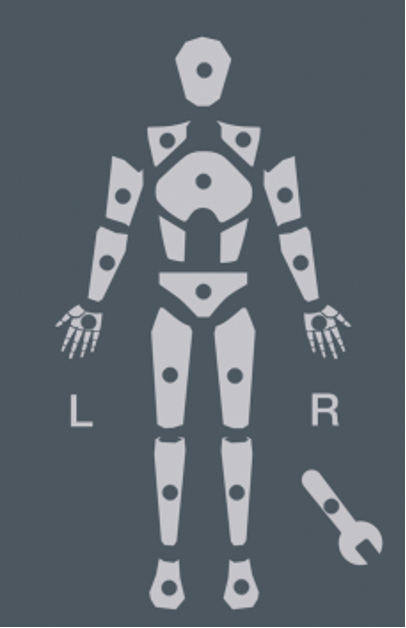
\includegraphics[width=3.5cm]{./images/sensors.png}
        \caption{加速度センサがついている位置}
        \label{sensors}
    \end{center}
\end{figure}
PERCEPTION NEURON 2.0は,図\ref{sensors}のような17点の位置にジャイロスコープ,加速度計,磁力計を備えたIMU(慣性計測装置)内蔵の加速度センサ(NEURON)を装着し,$x$,$y$,$z$軸方向の回転角度と推定位置座標をサンプリングレート120$\rm{Hz}$で時系列に採取する.
PERCEPTION NEURON 2.0を用いて採取した時系列データは,RAW,BVH(biovision hierarchical Data),FBX(Filebox)の形式に出力することが可能であるが,バイオメカニクスの視点で分析を行うことから,ヒトの骨格を階層構造としてモデリングしたBVHが適しているため,本研究ではBVHを採用する.
\begin{figure}
    \begin{center}
        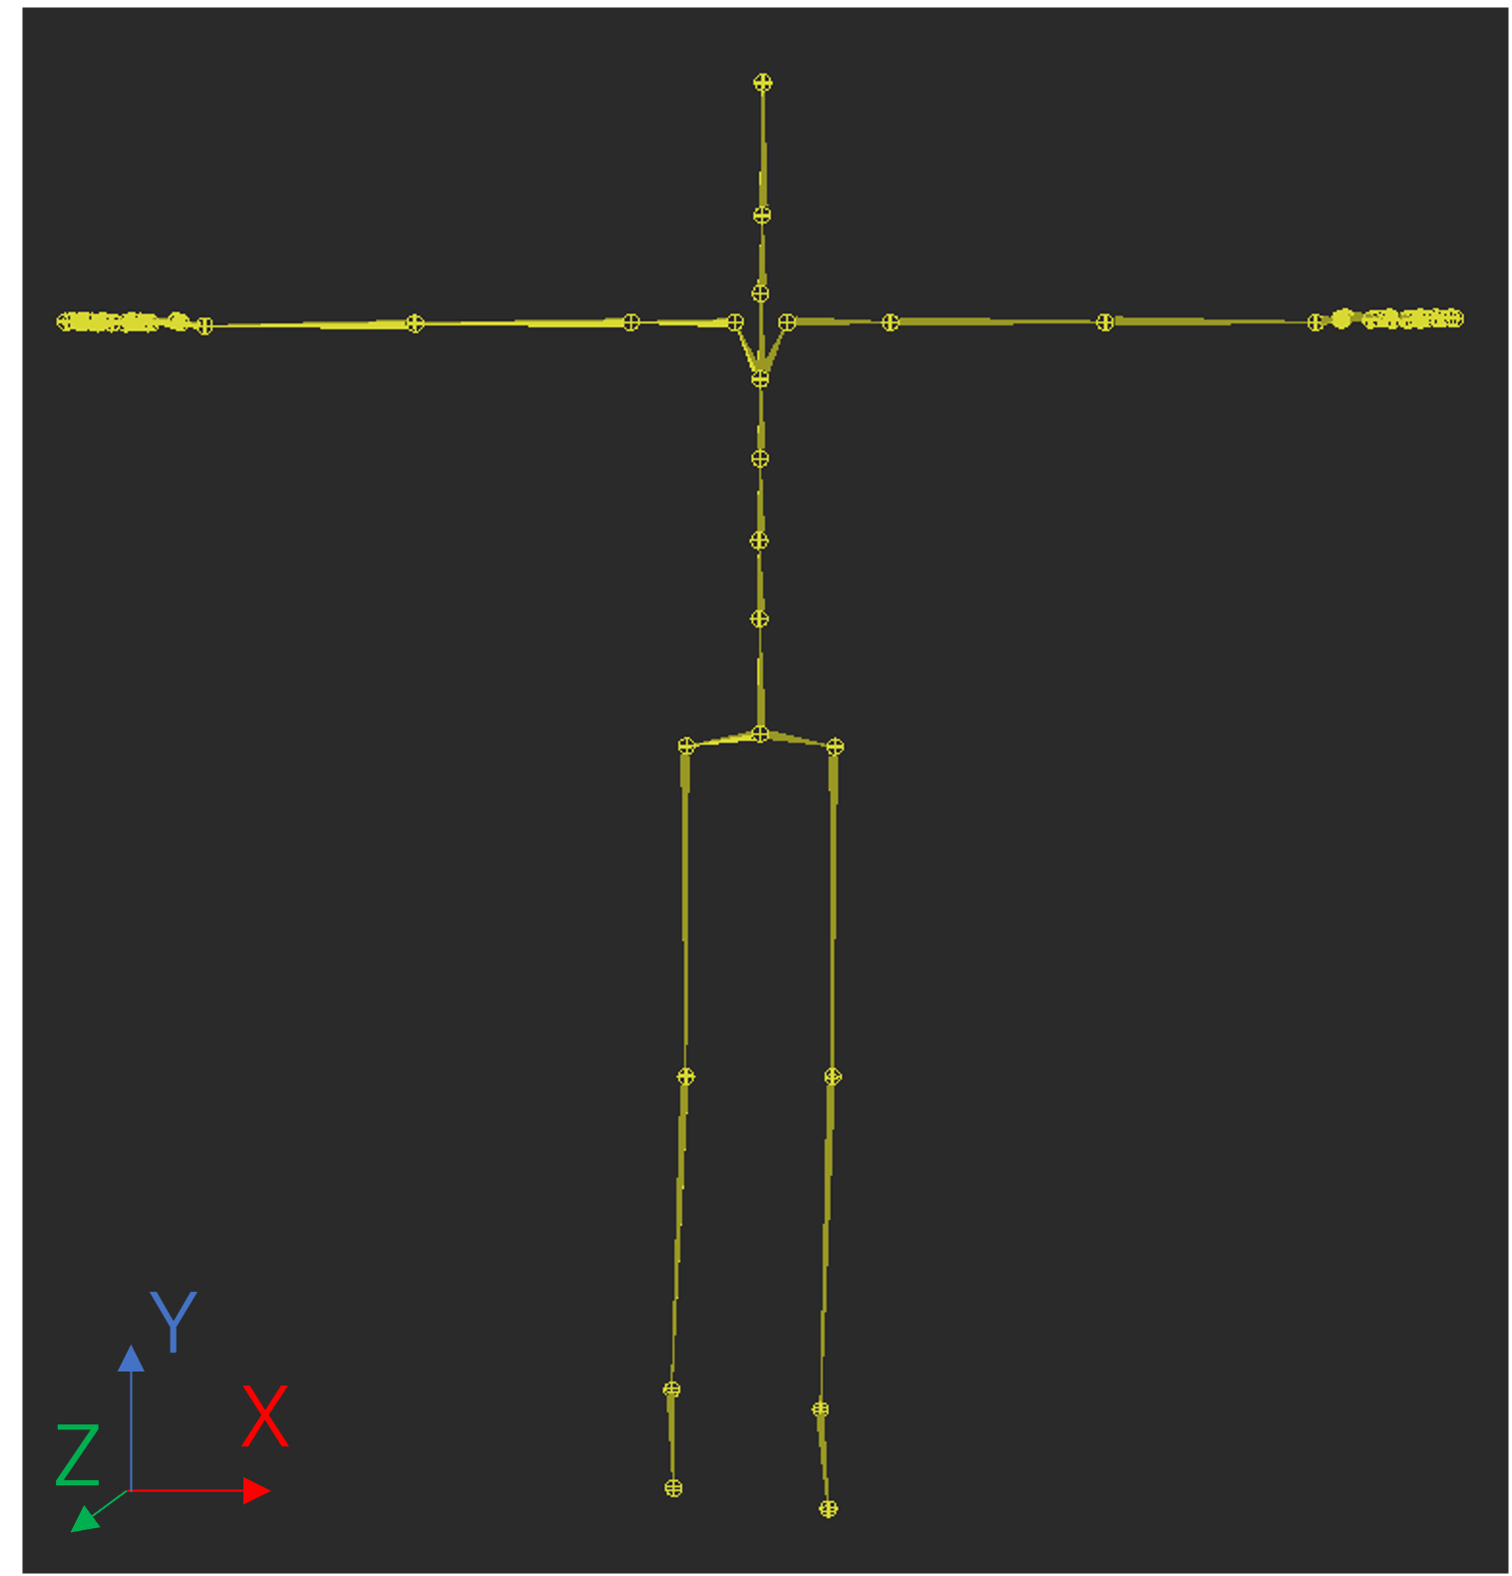
\includegraphics[width=5cm]{./images/Tpose.png}
        \caption{T-pose}
        \label{tpose}
    \end{center}
\end{figure}
BVHは,図\ref{tpose}のように59個の関節球の位置を計算し,$x$,$y$,$z$軸方向の回転角度とROOTである腰部の位置座標を時系列に書き出したファイル形式である.
PERCEPTION NEURON 2.0で採取される初めのデータ形式はRAW形式であるため,RAWからBVHへの変換は,PERCEPTION NEURON 2.0の専用ソフトであるAxis Neuronより行う.

図\ref{tpose}は,T-poseと呼ばれるデフォルトポーズである.
このポーズより$x$,$y$,$z$軸方向を定義し,各関節球の$x$,$y$,$z$軸方向の回転角度を0度とする.
BVHファイルに書き込まれている時系列データは,このポーズからの回転角を示し,ルートである腰部は$x$,$y$,$z$方向の位置座標も記録する.
よって,各関節球の3軸方向の回転角と腰部の3軸方向の位置座標を合計し,180チャンネルの時系列データを扱う.

%=================================================================================================================================================================================================================================%
\section{被験者情報}
被験者は,ゴルフ歴10年,平均スコア100のアベレージゴルファーである.
被験者にドライバーショットを行わせたところ,ストレート弾道に飛球したゴルフスイング動作,スライス弾道でヘッドアップ動作をしたゴルフスイング動作,スライス弾道で身体が開く動作をしたゴルフスイング動作の3種類の動作を採取することができ,各動作で6スイングずつの時系列データを採取した.
各時系列データごとにHHTを適用させたところ,4から6個のIMFと残差に分解した.
本研究では,各IMF毎に瞬時周波数と瞬時振幅を求め,瞬時周波数$f$,瞬時振幅$A$は以下の式のように処理をした.

\begin{equation}
    f_{ave}(t) = \frac{1}{n} \sum_{k=1}^{n} f_{k}
\end{equation}

\begin{equation}
    \tilde{A}(t) = \sqrt{\sum_{k=1}^{n} A_{k}}
\end{equation}

本研究では,アベレージゴルファーのスライスの原因としてよく挙げられるヘッドアップ動作,身体が開く動作をしたゴルフスイングに注目し,ストレート弾道に飛球したゴルフスイングと比較して考察を行う.

%=================================================================================================================================================================================================================================%
\section{スペクトログラム解析}
%=================================================================================================================================================================================================================================%
\subsection{頸部,左膝モーションのIMF1}
\begin{figure}
    \begin{center}
        \begin{tabular}{c}
            \begin{minipage}{0.5\hsize}
                \begin{center}
                    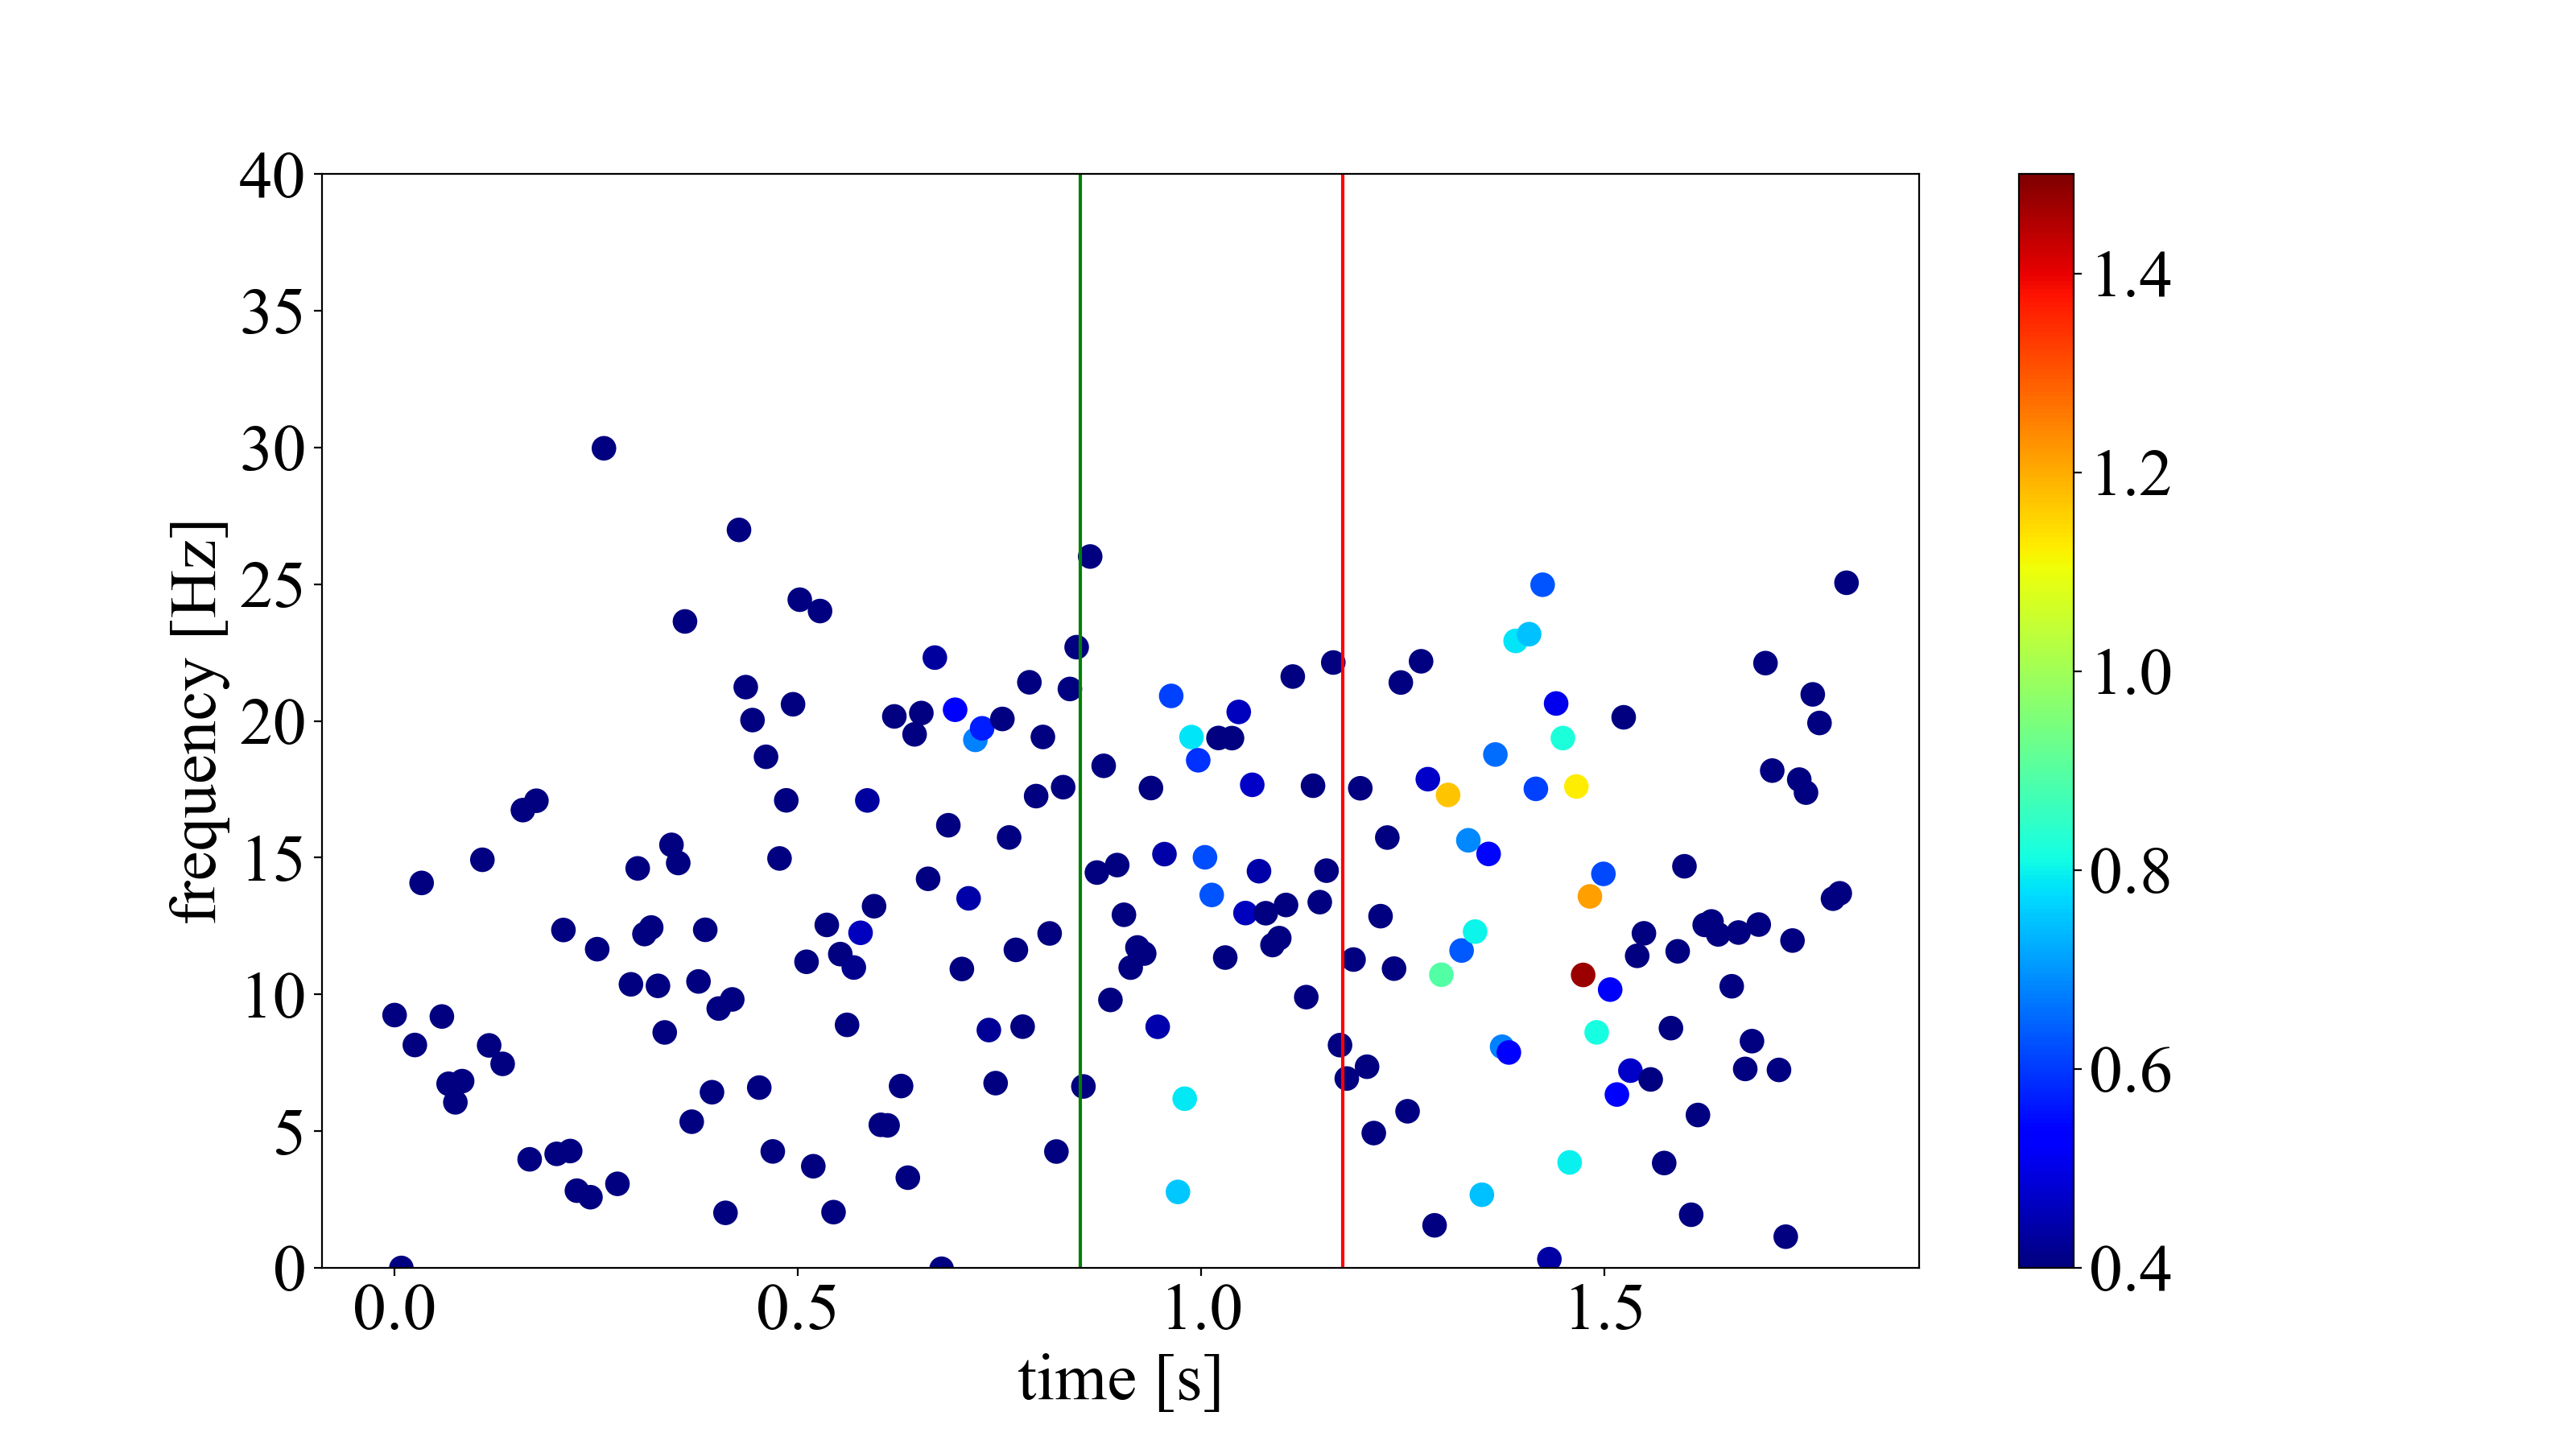
\includegraphics[width=8cm]{./images/straight_data/neck/IMF1.png}
                    % \caption{ストレート弾道で頸部モーションIMF1}
                    (a)
                    \label{straight neck imf1}
                \end{center}
            \end{minipage}

            \begin{minipage}{0.5\hsize}
                \begin{center}
                    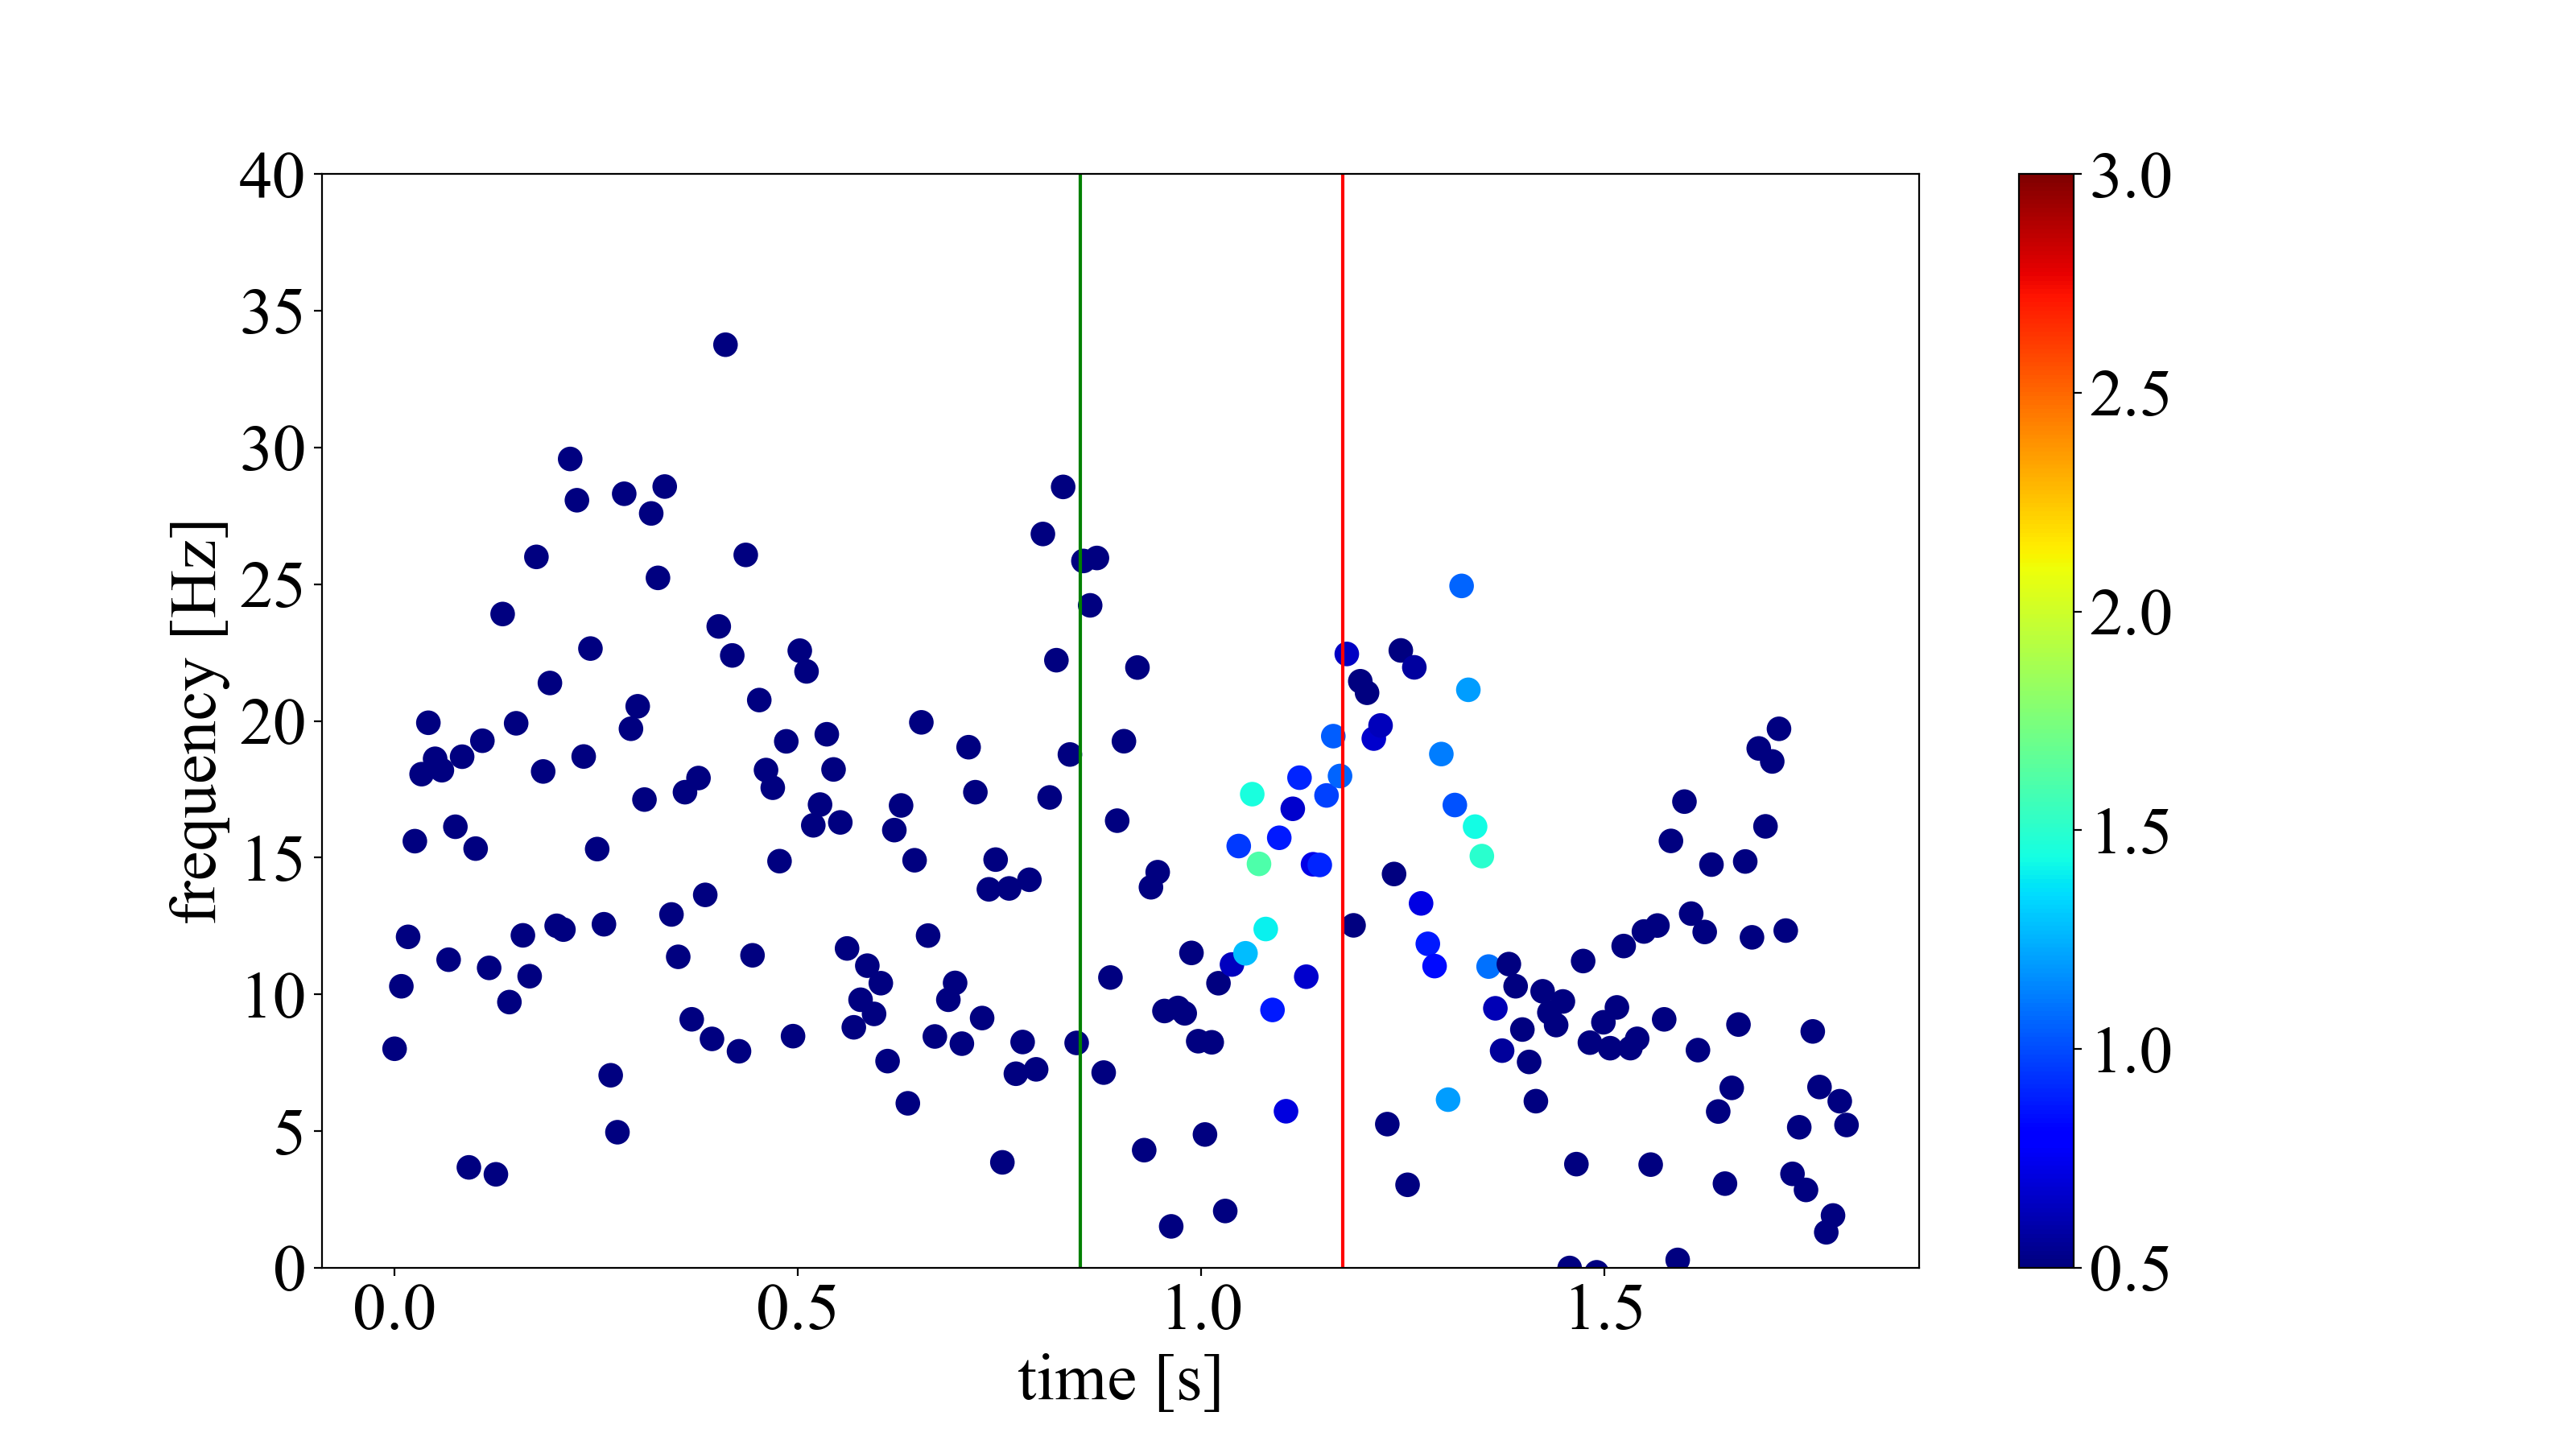
\includegraphics[width=8cm]{./images/straight_data/left_leg/IMF1.png}
                    % \caption{ストレート弾道で左膝モーションIMF1}
                    (b)
                    \label{straight left leg imf1}
                \end{center}
            \end{minipage}
        \end{tabular}
    \end{center}

    \begin{center}
        \begin{tabular}{c}
            \begin{minipage}{0.5\hsize}
                \begin{center}
                    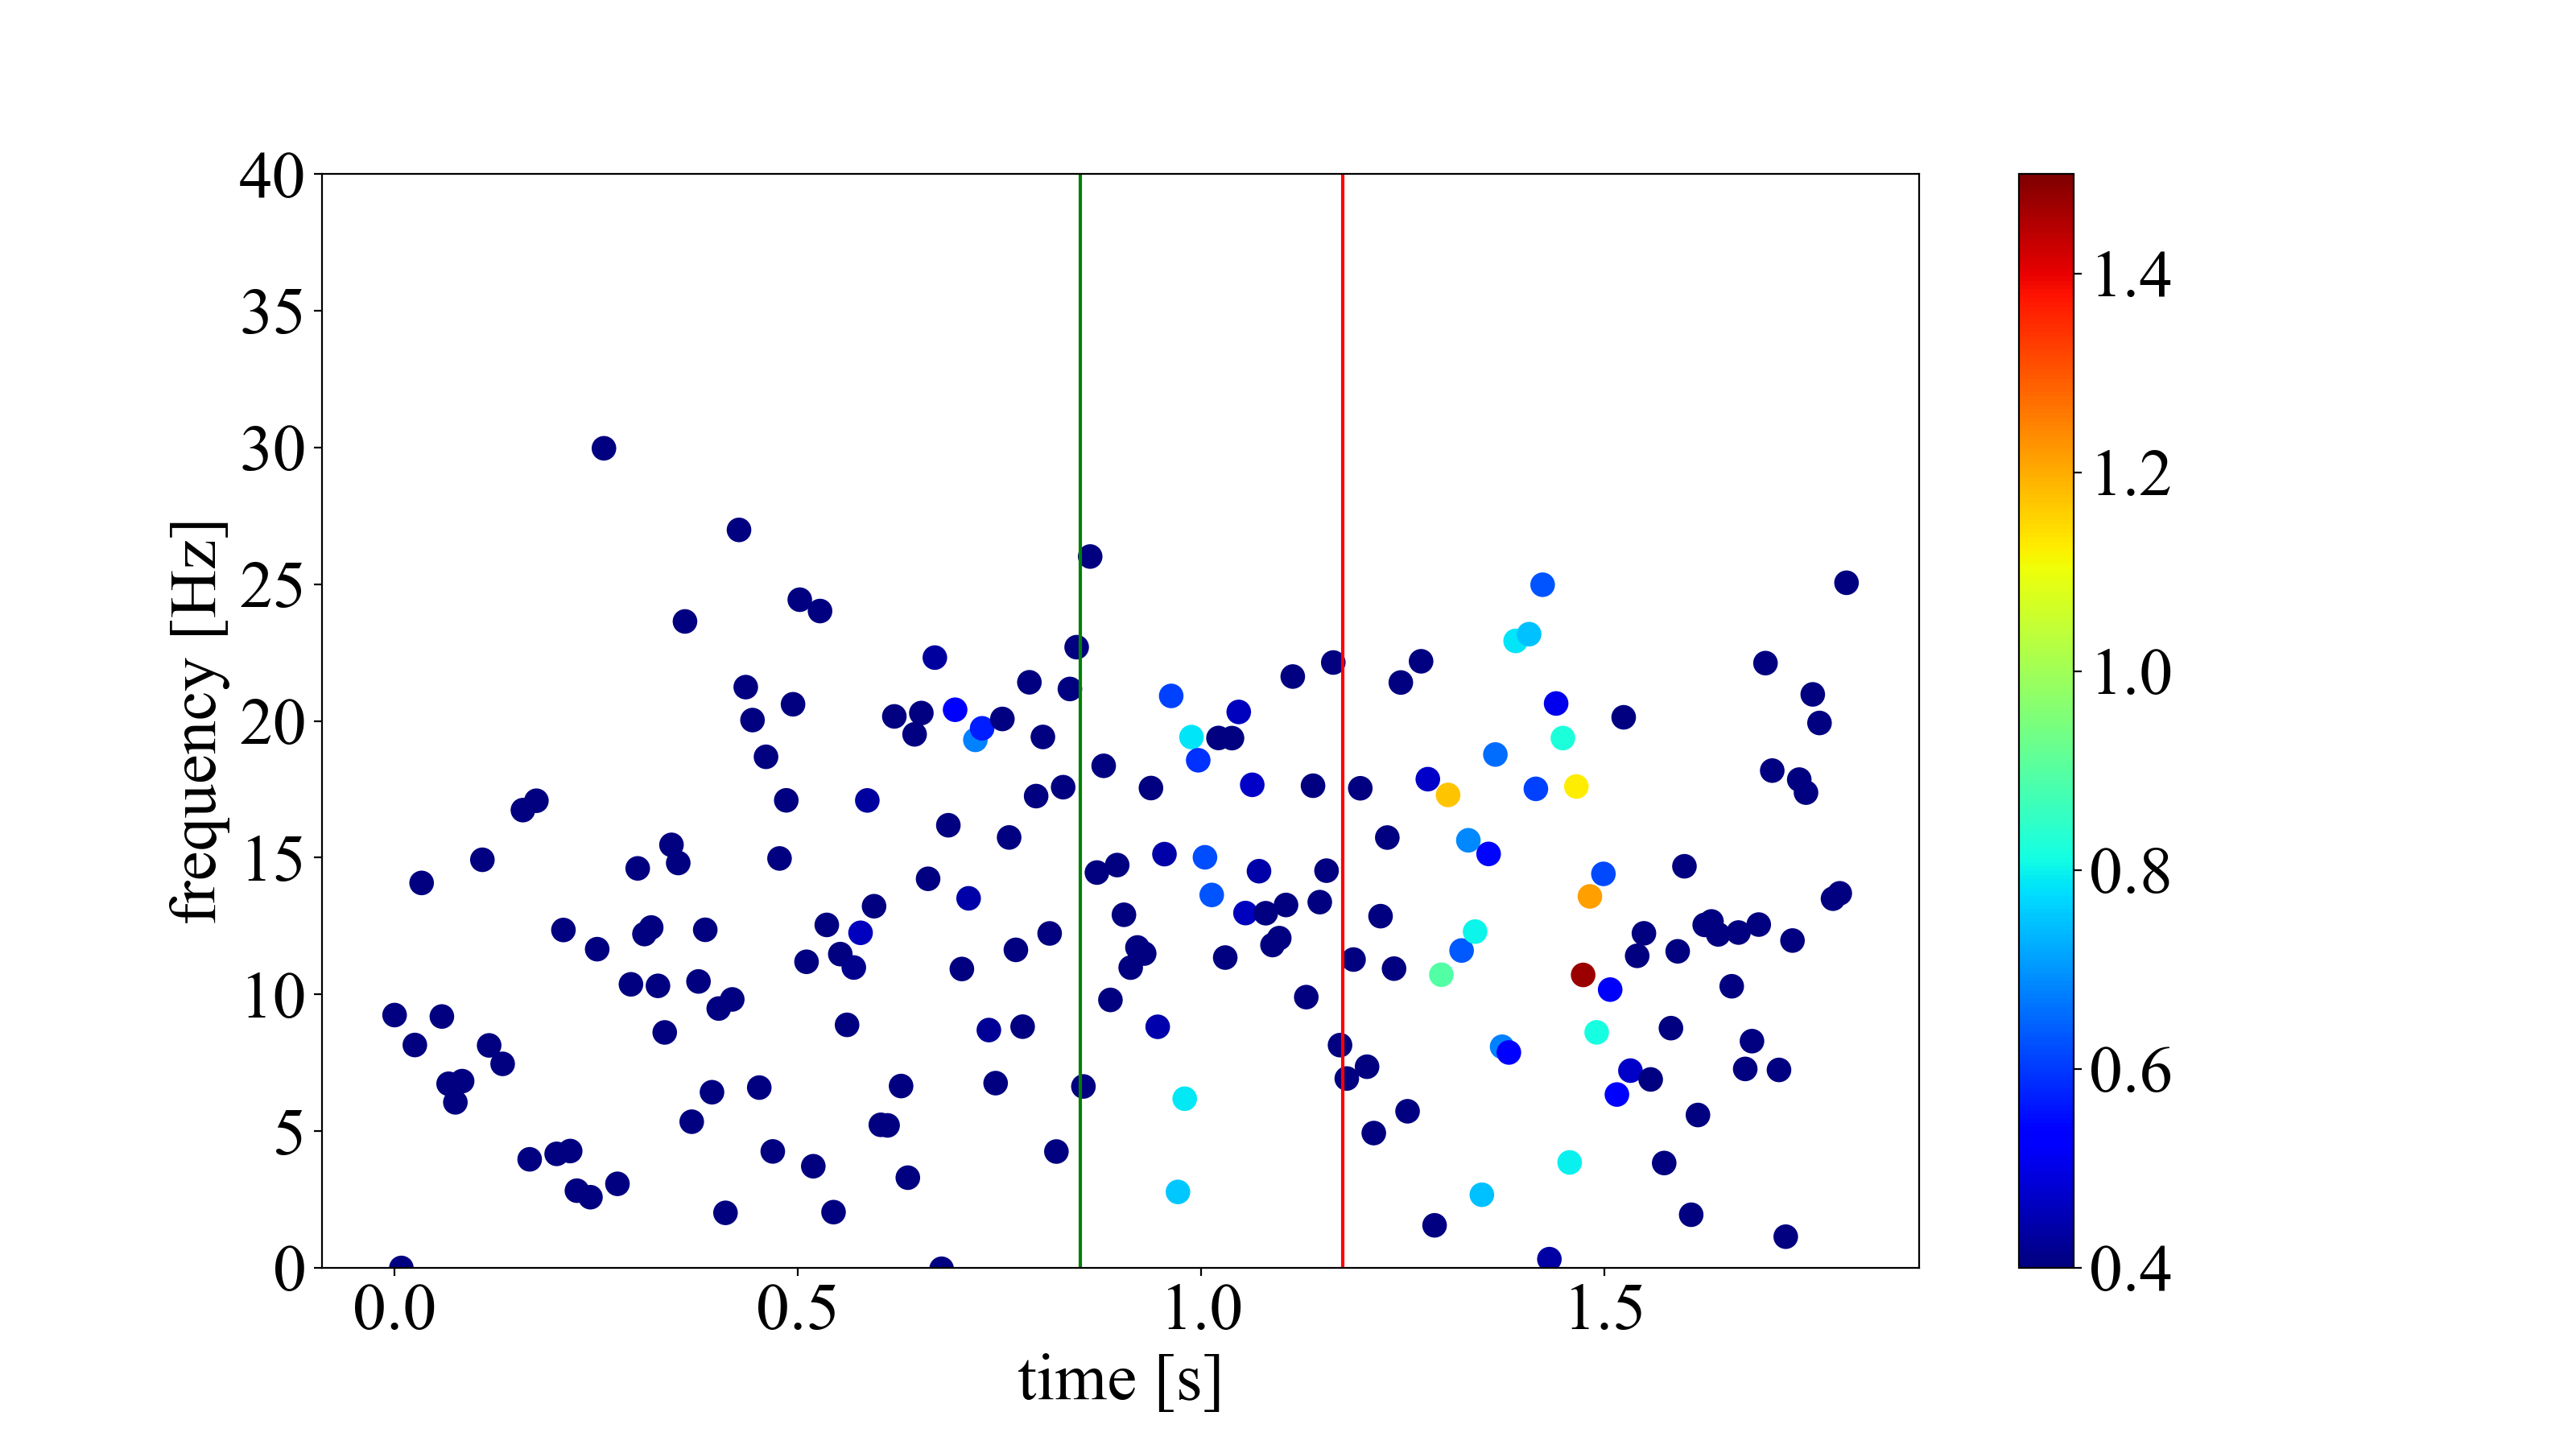
\includegraphics[width=8cm]{./images/straight_data/neck/IMF1.png}
                    % \caption{スライス弾道で頸部モーションIMF1}
                    (c)
                    \label{slice neck imf1}
                \end{center}
            \end{minipage}

            \begin{minipage}{0.5\hsize}
                \begin{center}
                    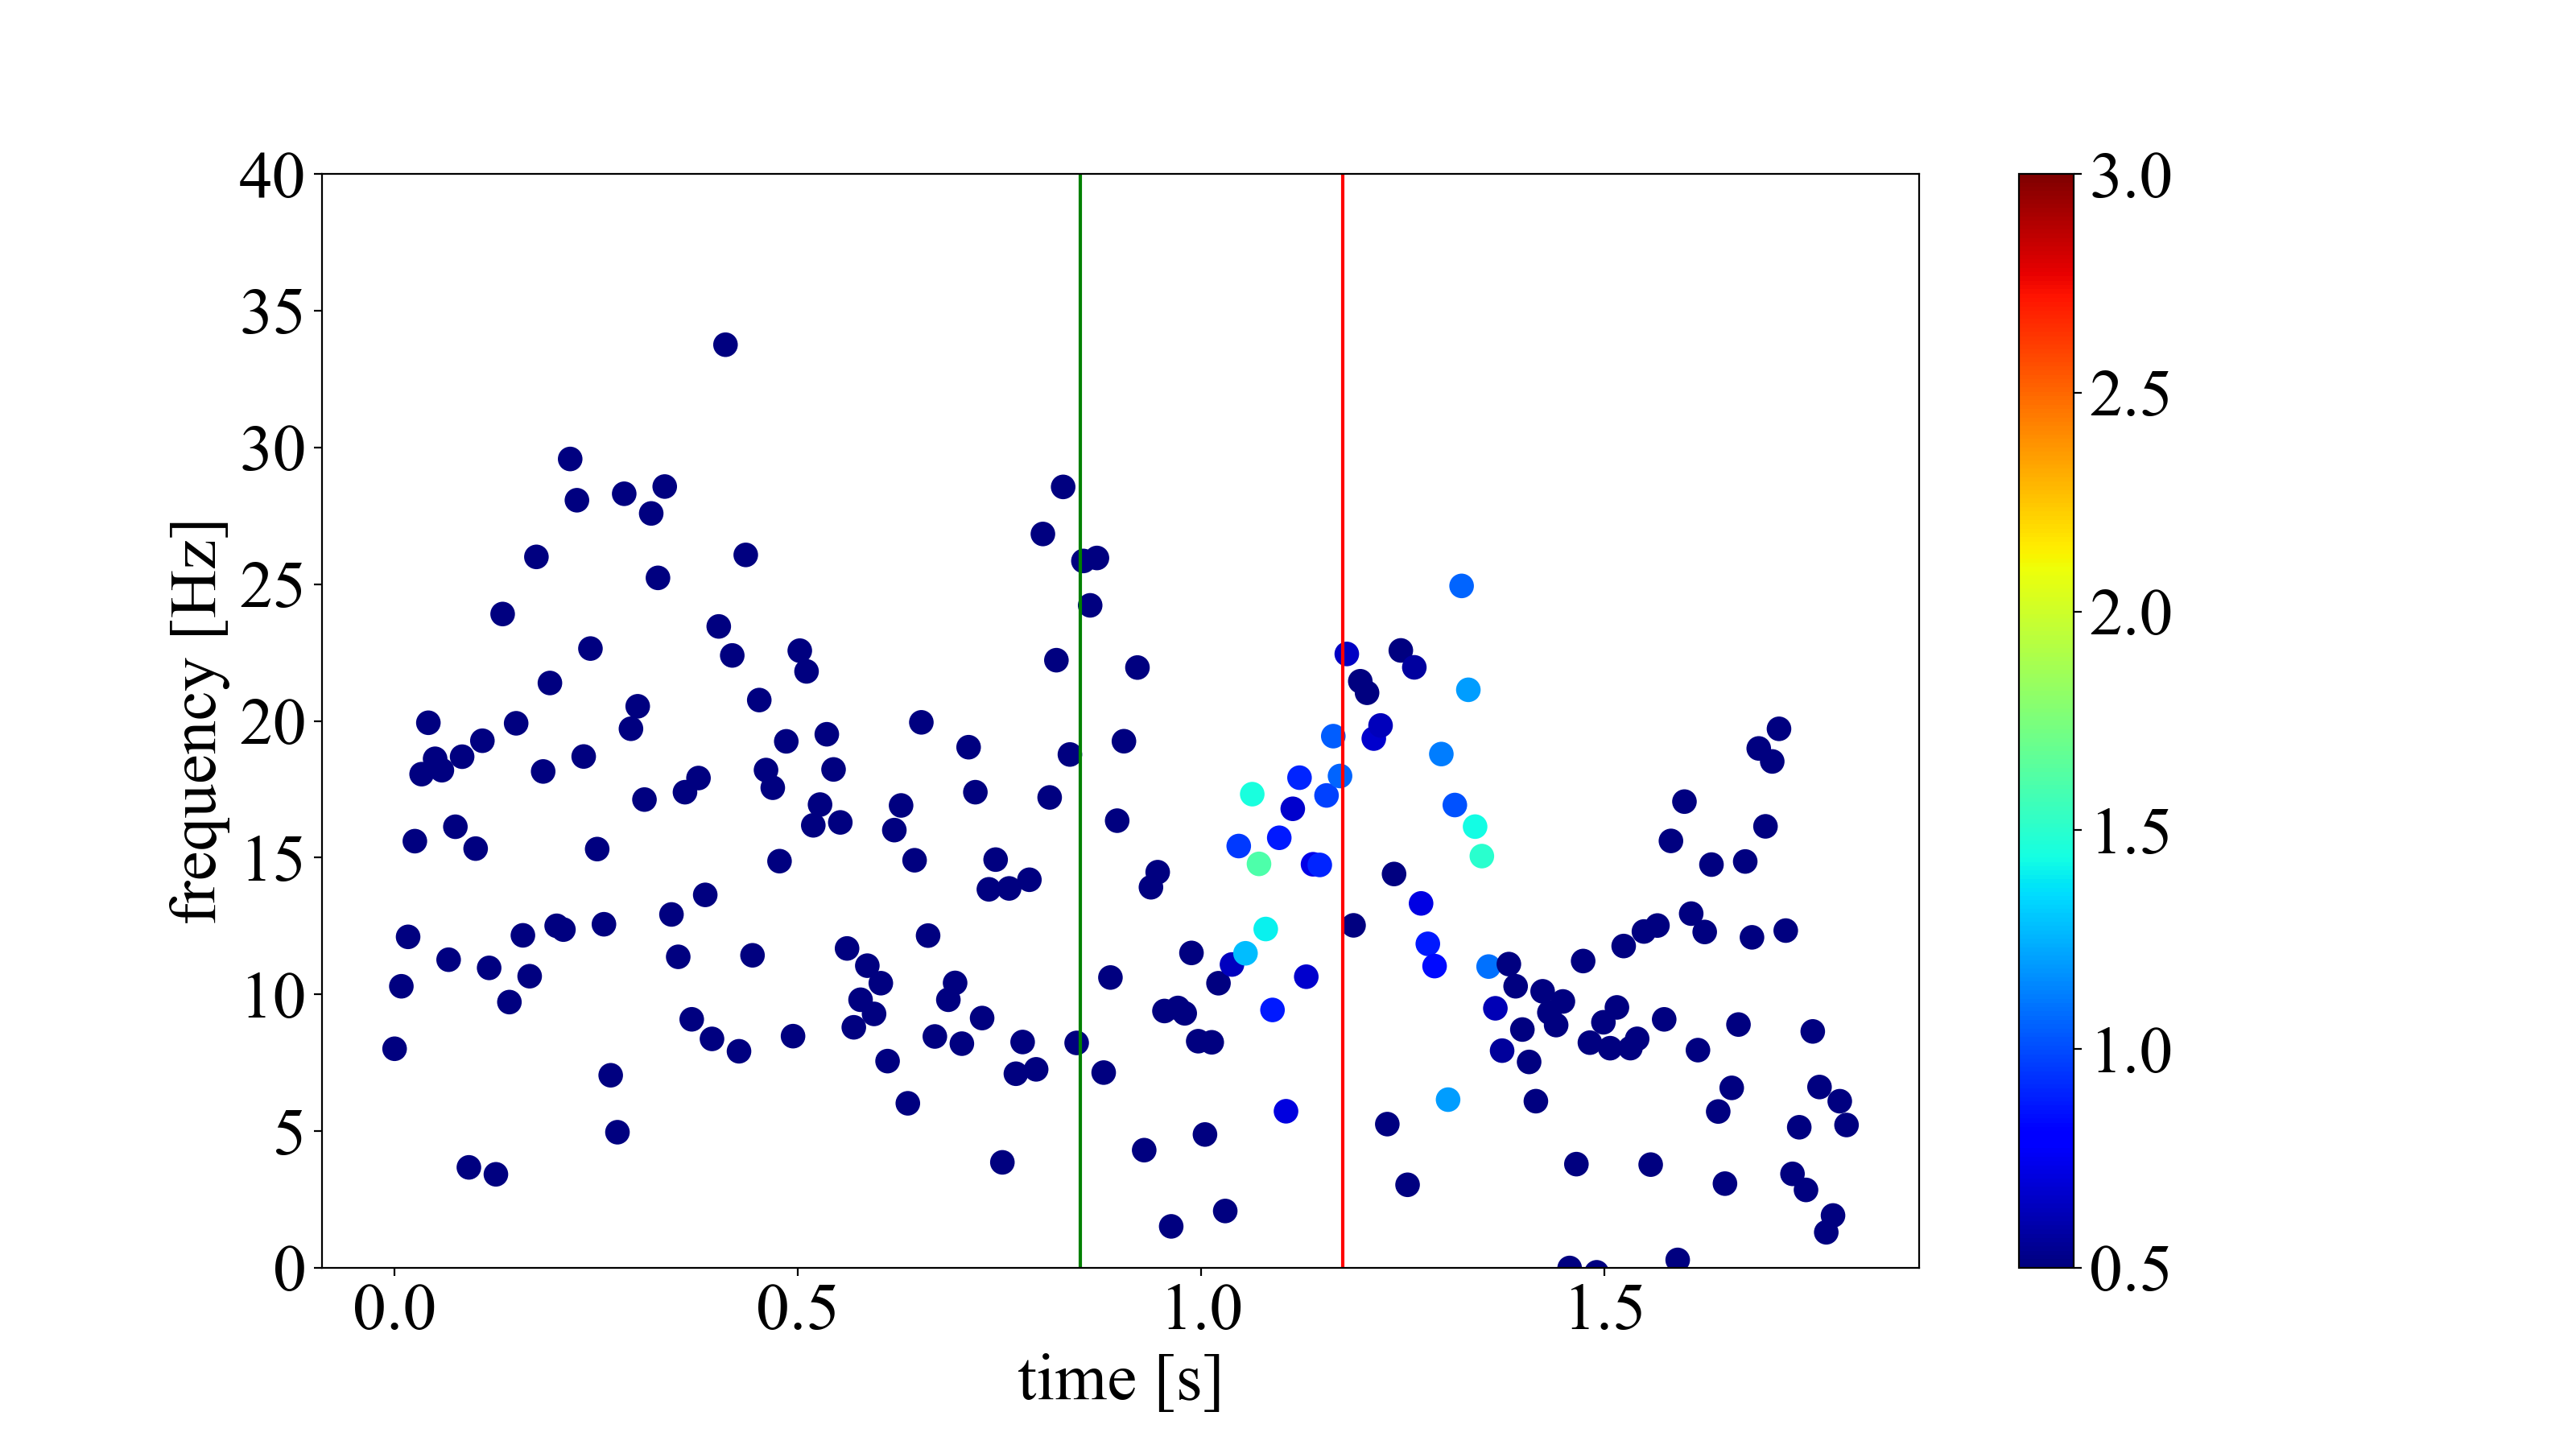
\includegraphics[width=8cm]{./images/straight_data/left_leg/IMF1.png}
                    % \caption{スライス弾道で左膝モーションIMF1}
                    (d)
                    \label{slice left leg imf1}
                \end{center}
            \end{minipage}
        \end{tabular}
    \end{center}
    \caption{ストレート弾道,スライス弾道に飛球した頸部,左膝モーションIMF1のスペクトログラム.(a)はストレート弾道で頸部モーションIMF1.(b)はストレート弾道で左膝モーションIMF1.(c)はスライス弾道で頸部モーションIMF1.(d)はスライス弾道で左膝モーションIMF1.}
    \label{imf1}
\end{figure}

% 被験者のドライバーショットを数値化し,ストレート弾道,ヘッドアップ動作をしたスライス弾道,身体が開く動作をしたスライス弾道の3つに分類し,各分類毎ヒルベルト・ファン変換を適用させ,瞬時周波数と瞬時振幅を計算した.
図\ref{imf1}は,ストレート弾道,スライス弾道に飛球したゴルフスイングモーションにHHTを適用させ,各弾道の頸部モーション,左膝モーションのIMF1をスペクトログラムにしたものある.
図\ref{imf1}の縦軸は瞬時周波数,横軸は時間,カラーバーは瞬時振幅(度),赤線はインパクト,緑線はトップを示している.
IMF1のスペクトログラムでは,瞬時周波数がおよそ$0\rm{Hz}$から$30\rm{Hz}$帯,瞬時振幅はおよそ0.4度から0.6度で離散的に分布されていることが確認できる.
すなわち,高周波成分のスペクトログラムでは,ストレート弾道とスライス弾道となる原因を示すことが難しい.

%=================================================================================================================================================================================================================================%
\subsection{ヘッドアップ動作}
\begin{figure}
    \begin{center}
        \begin{tabular}{c}
            \begin{minipage}{0.5\hsize}
                \begin{center}
                    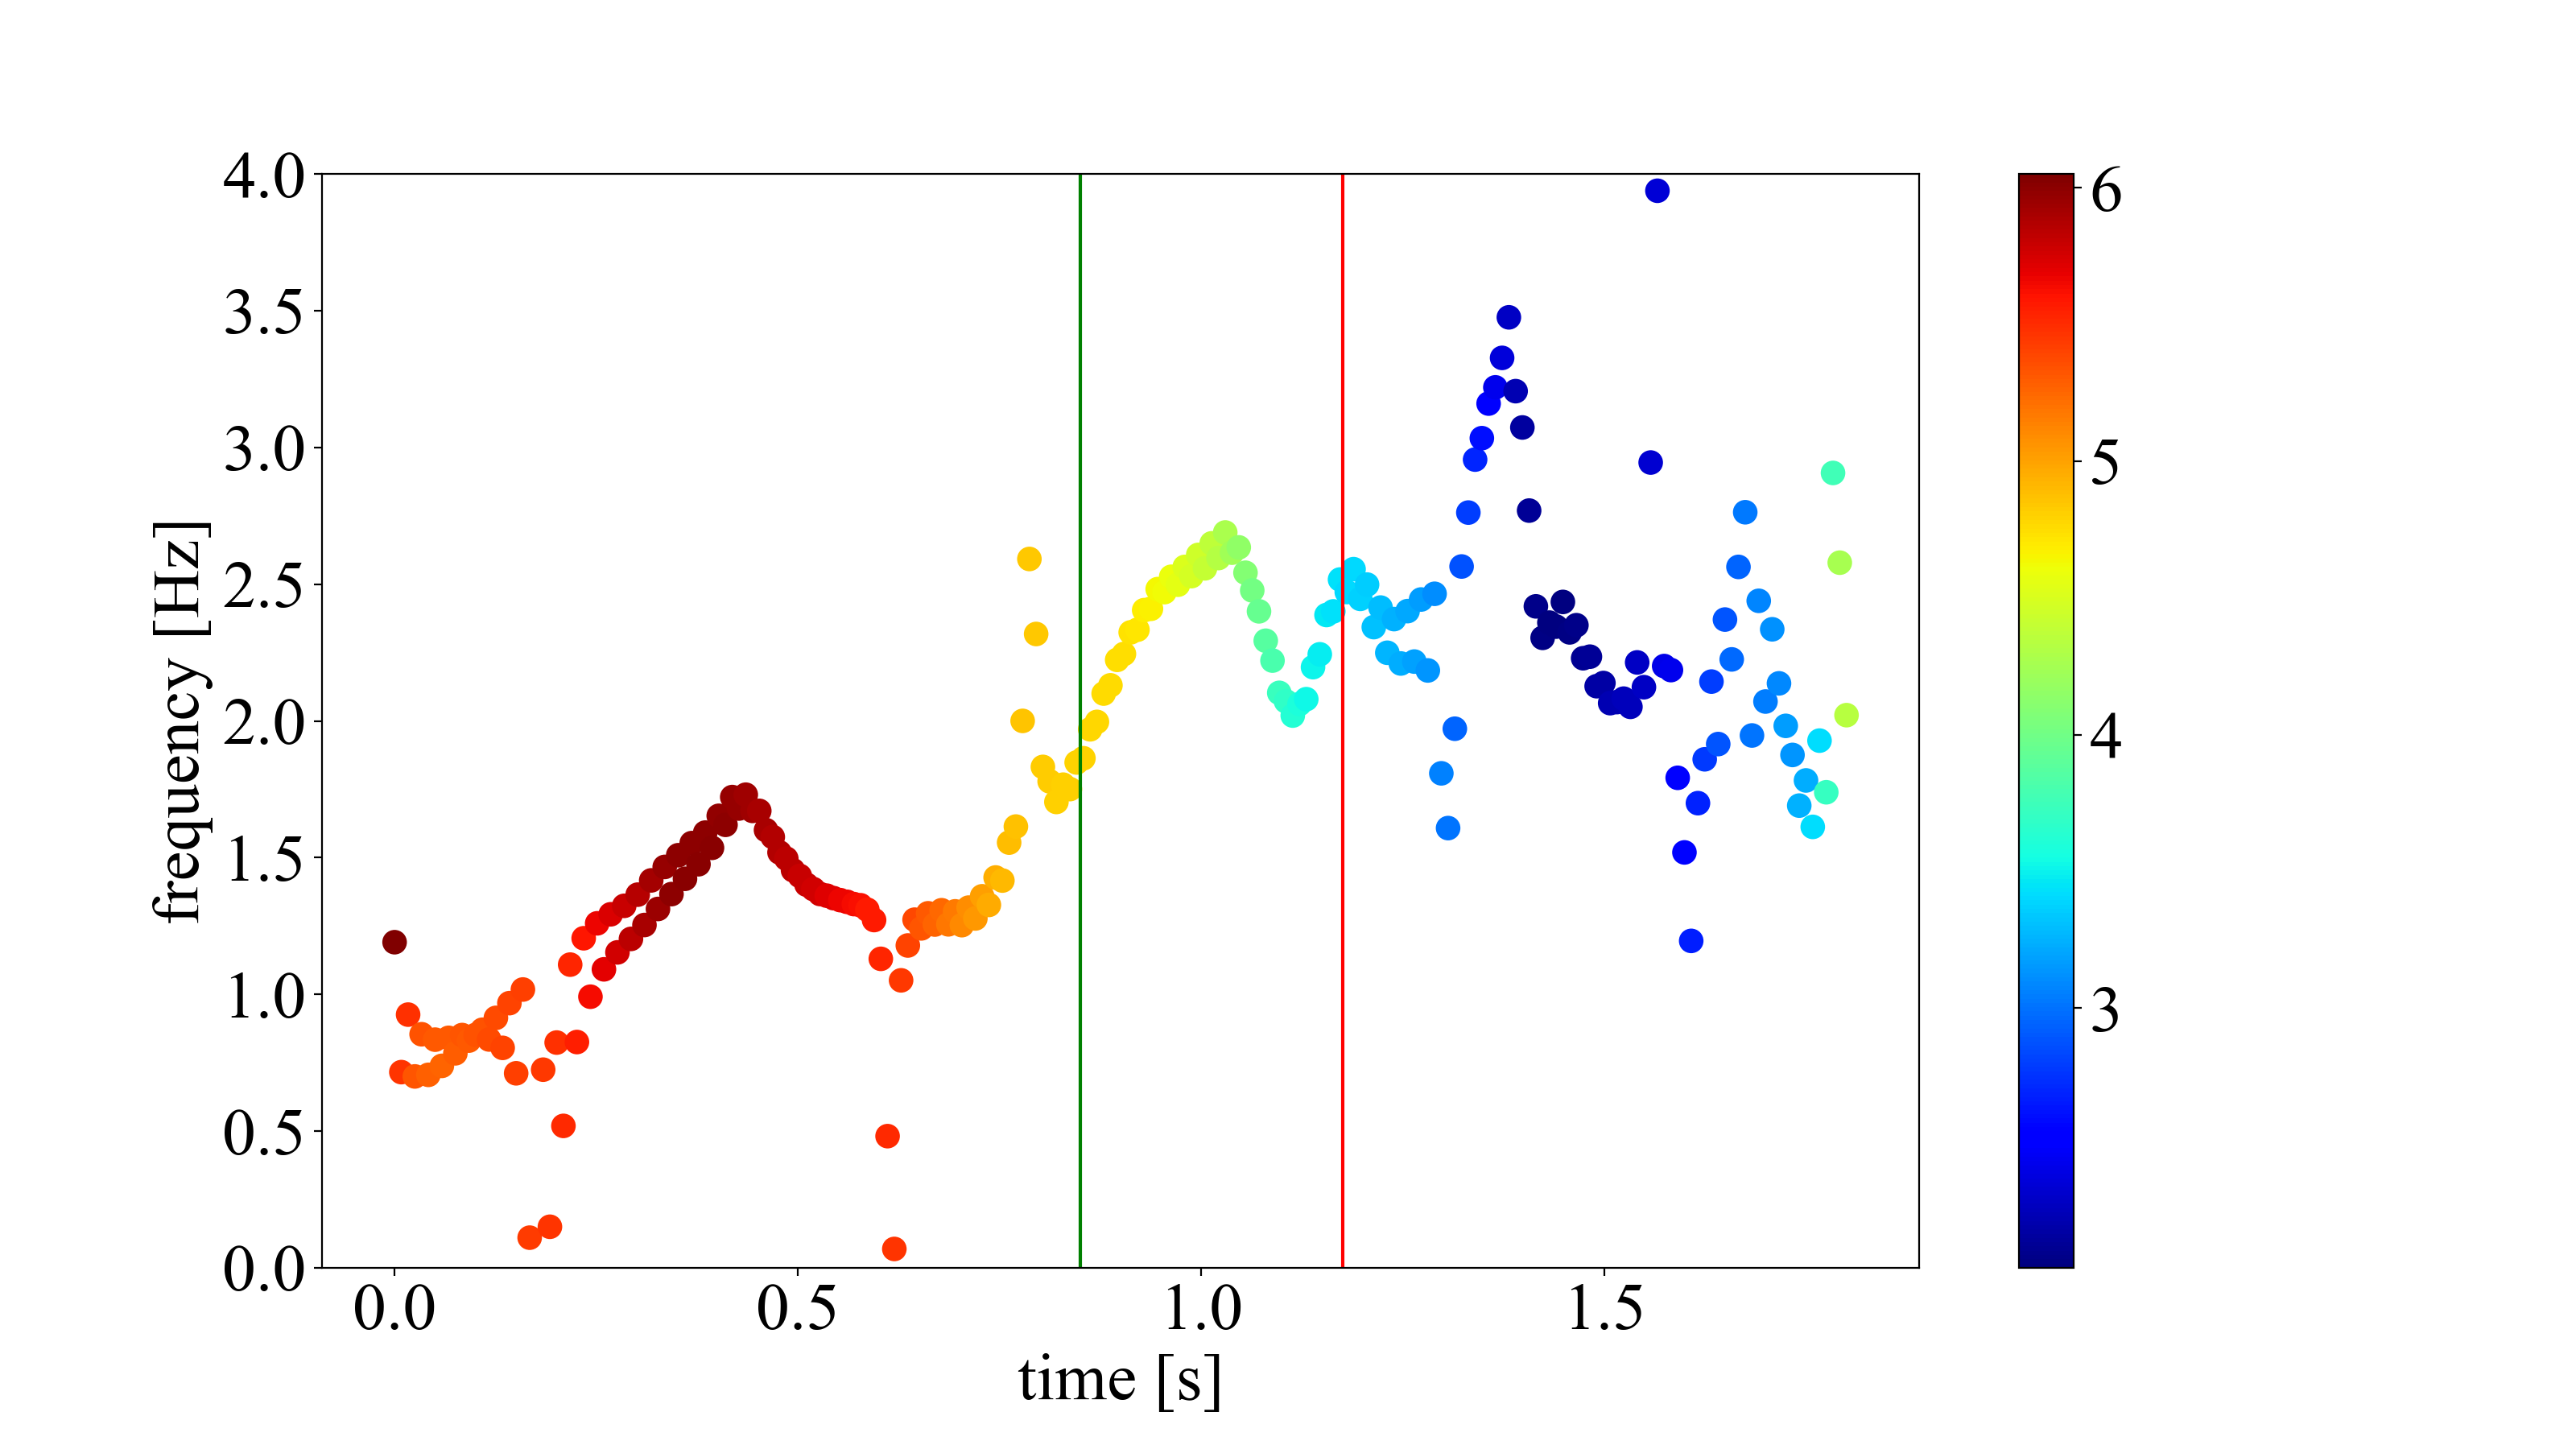
\includegraphics[width=8cm]{./images/straight_data/neck/IMF4.png}
                    (e)
                \end{center}
            \end{minipage}

            \begin{minipage}{0.5\hsize}
                \begin{center}
                    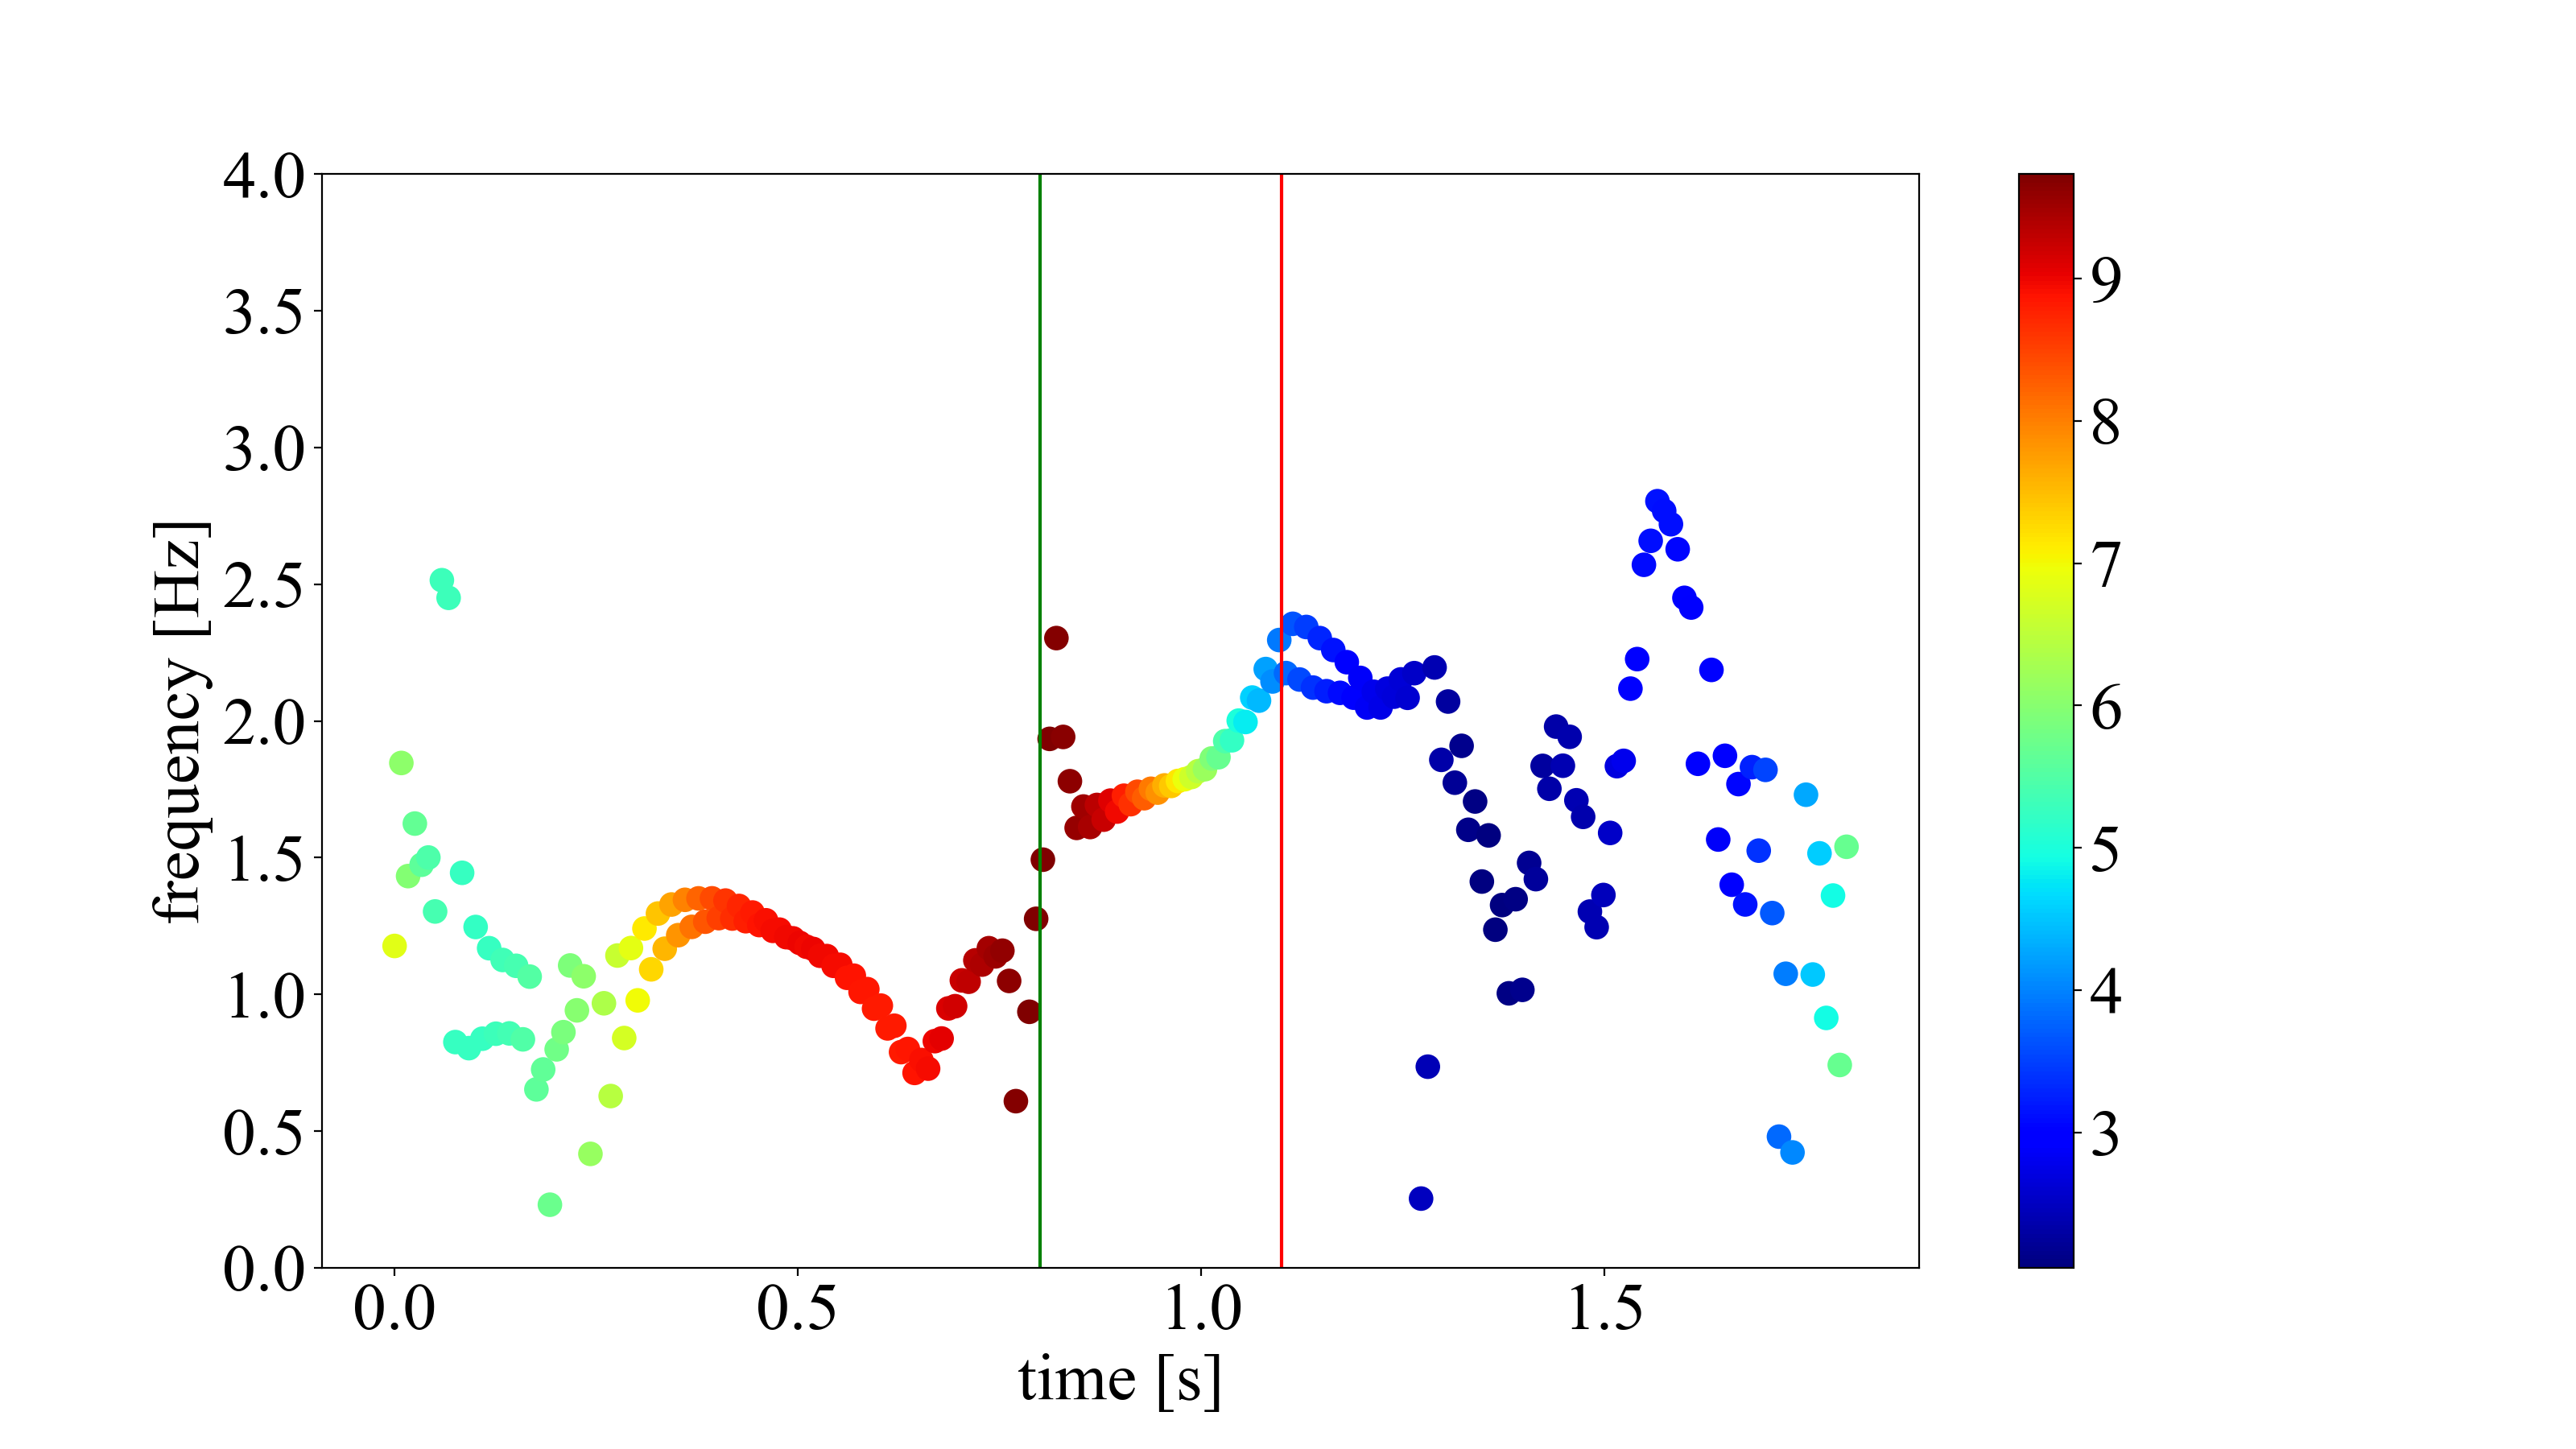
\includegraphics[width=8cm]{./images/headup_data/neck/IMF4.png}
                    (f)
                \end{center}
            \end{minipage}
        \end{tabular}
    \end{center}
    \caption{ストレート弾道,スライス弾道に飛球した頸部モーションIMF4のスペクトログラム.(e)はストレート弾道の頸部モーションIMF4.(f)はスライス弾道の頸部モーションIMF4.}
\end{figure}

%=================================================================================================================================================================================================================================%
\subsection{身体が開く動作}
\begin{figure}
    \begin{center}
        \begin{tabular}{c}
            \begin{minipage}{0.5\hsize}
                \begin{center}
                    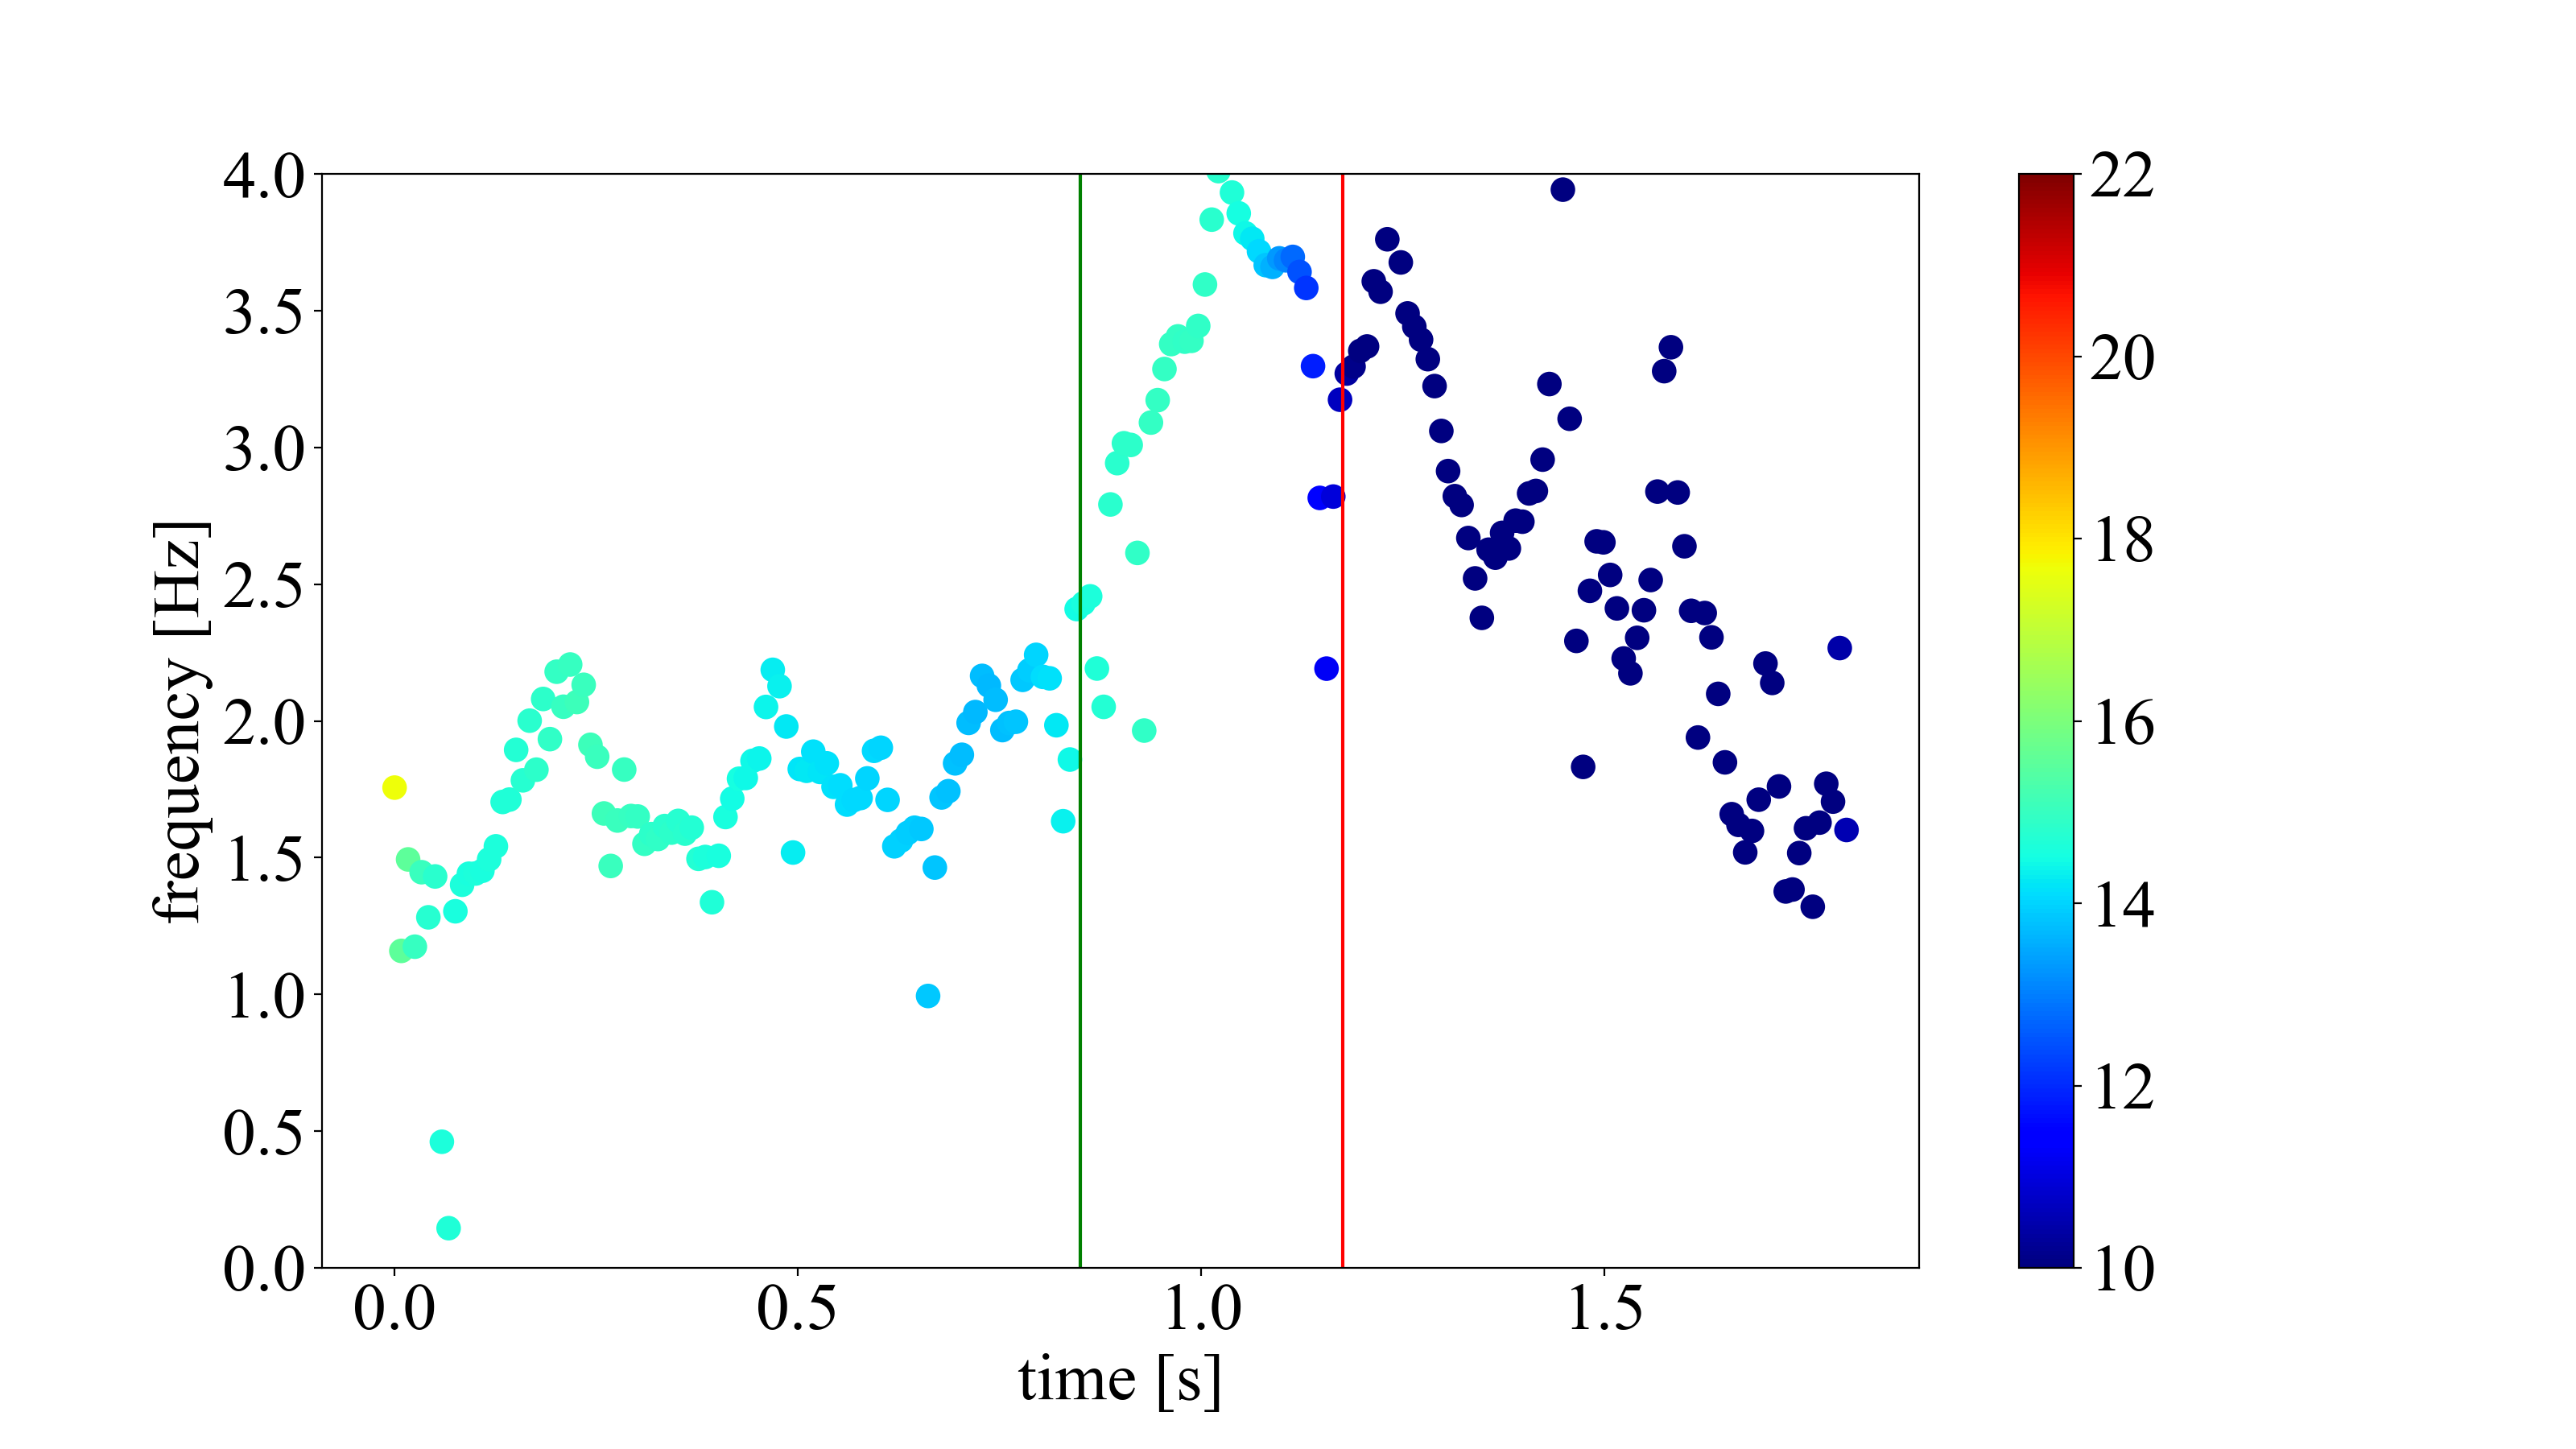
\includegraphics[width=8cm]{./images/straight_data/left_up_leg/IMF4.png}
                    (g)
                \end{center}
            \end{minipage}

            \begin{minipage}{0.5\hsize}
                \begin{center}
                    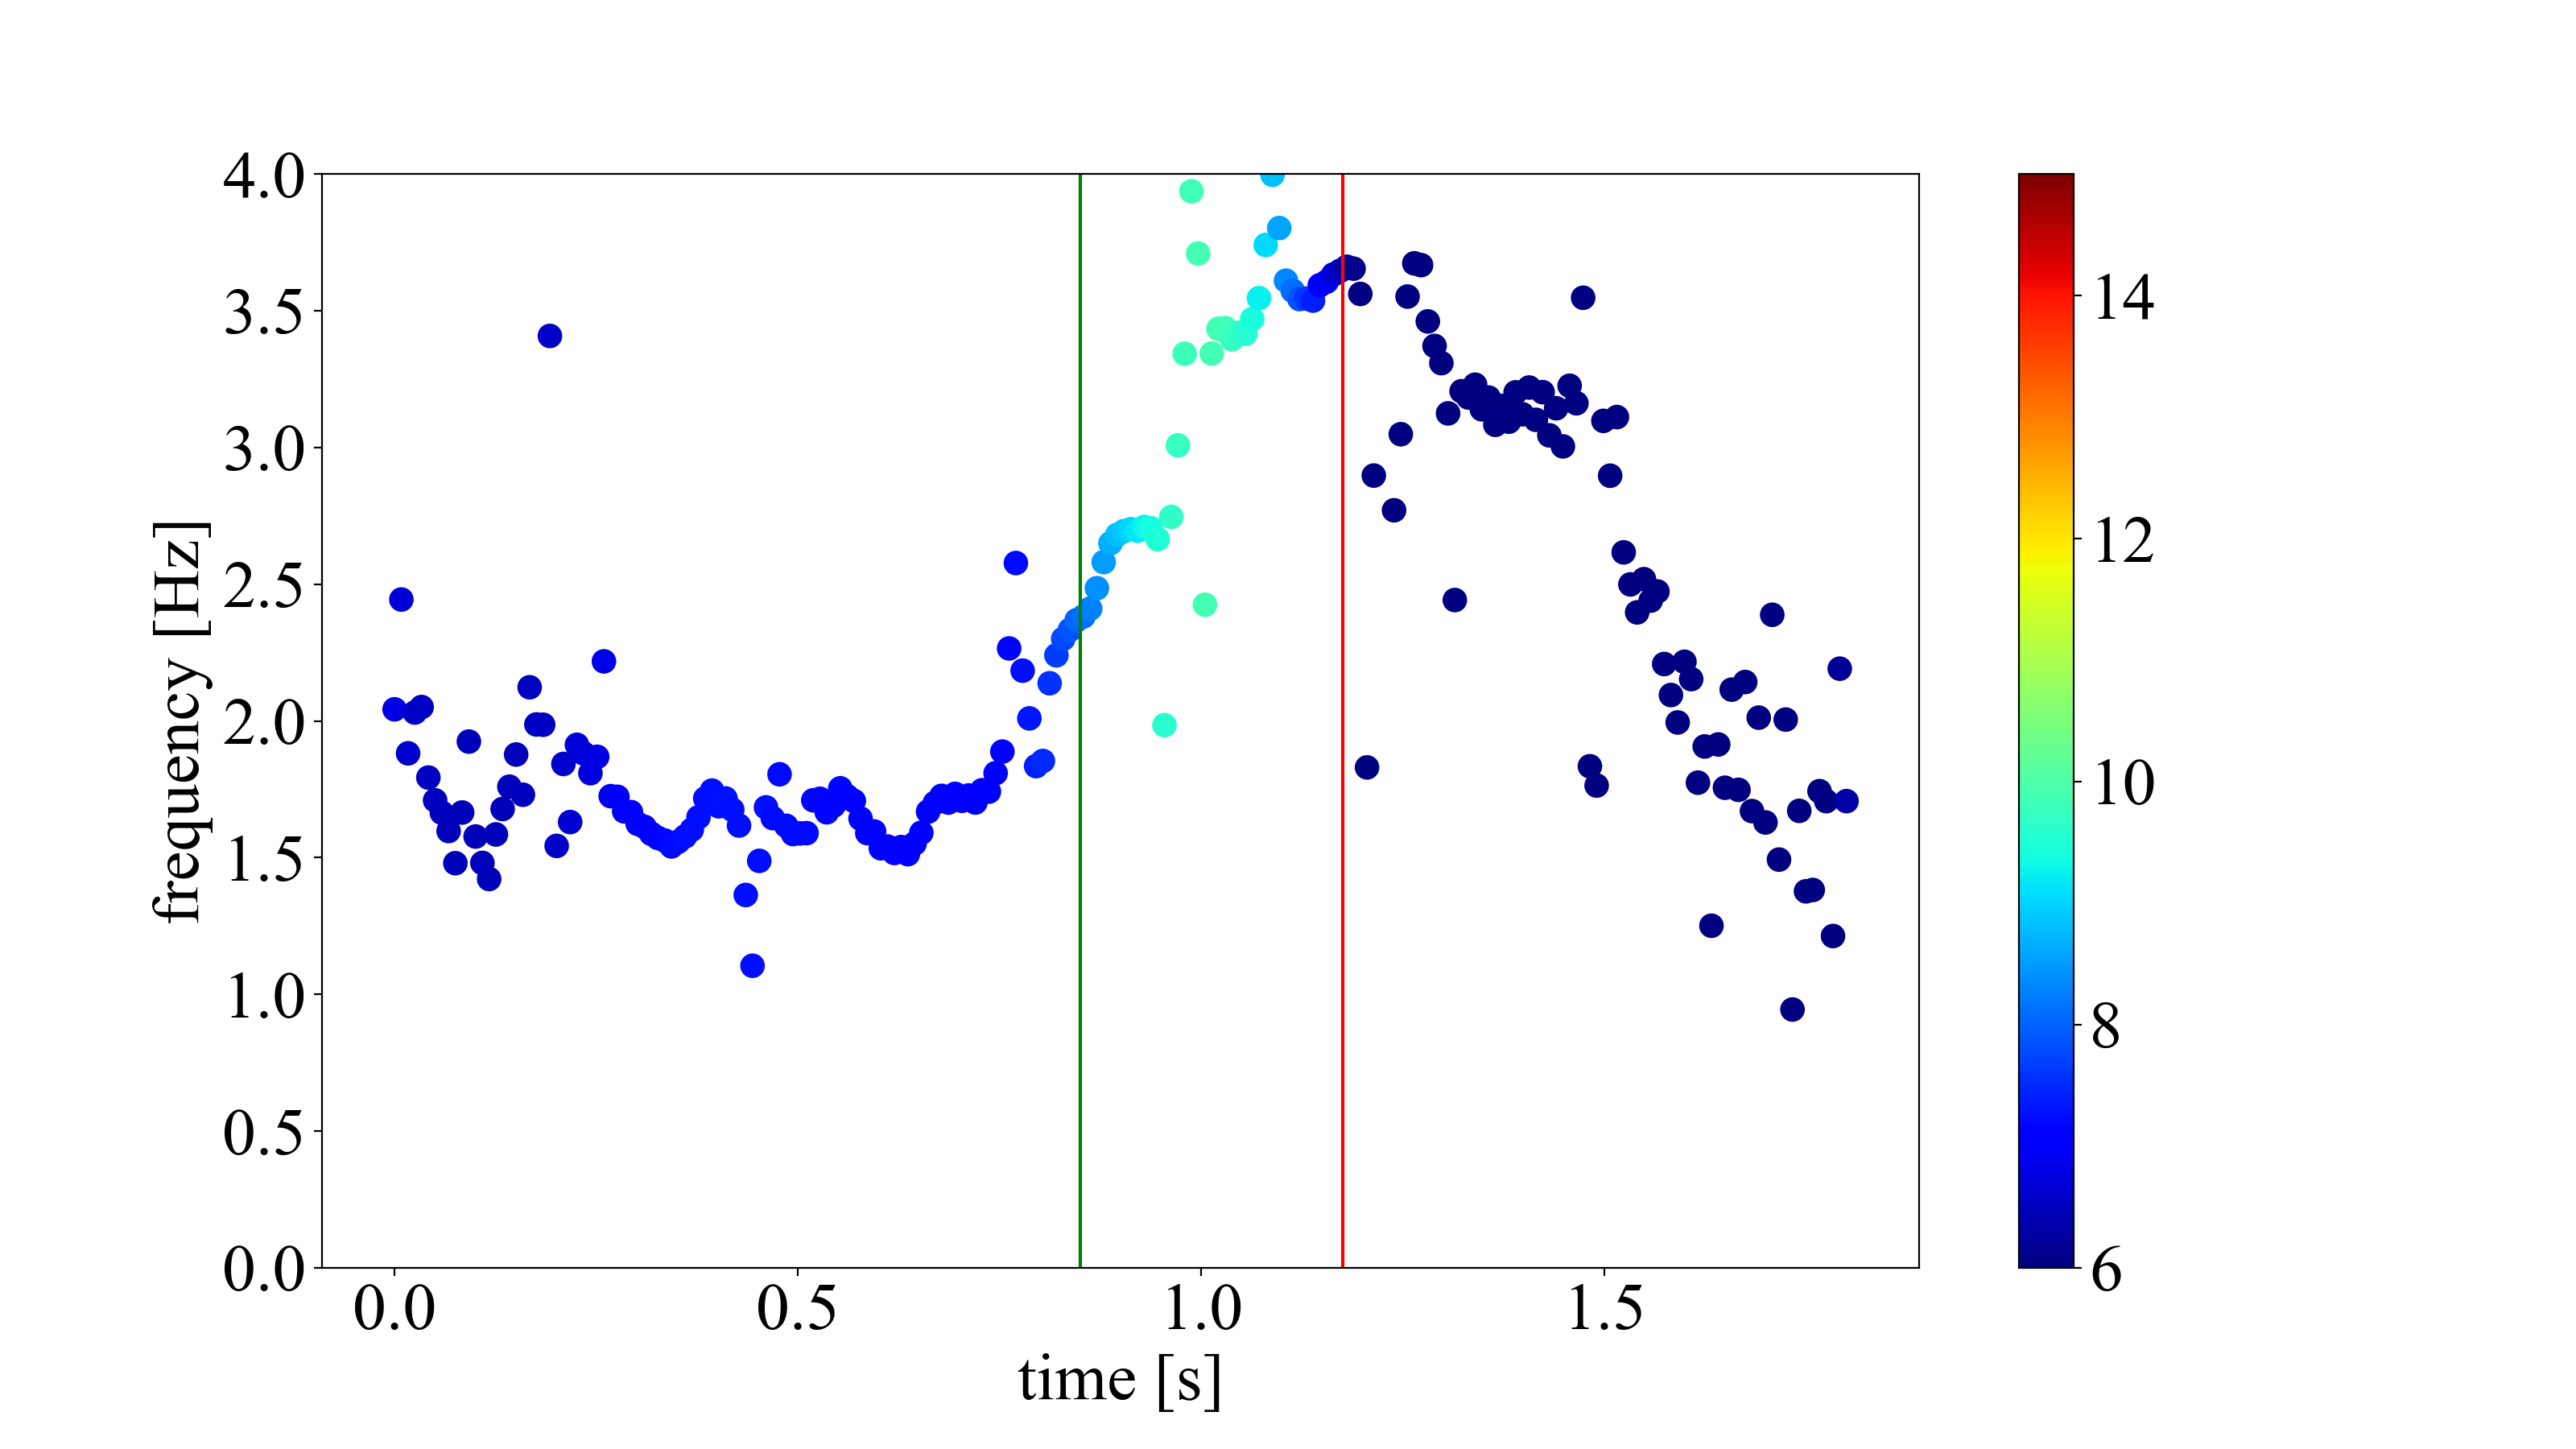
\includegraphics[width=8cm]{./images/straight_data/left_leg/IMF4.png}
                    (h)
                \end{center}
            \end{minipage}
        \end{tabular}
    \end{center}

    \begin{center}
        \begin{tabular}{c}
            \begin{minipage}{0.5\hsize}
                \begin{center}
                    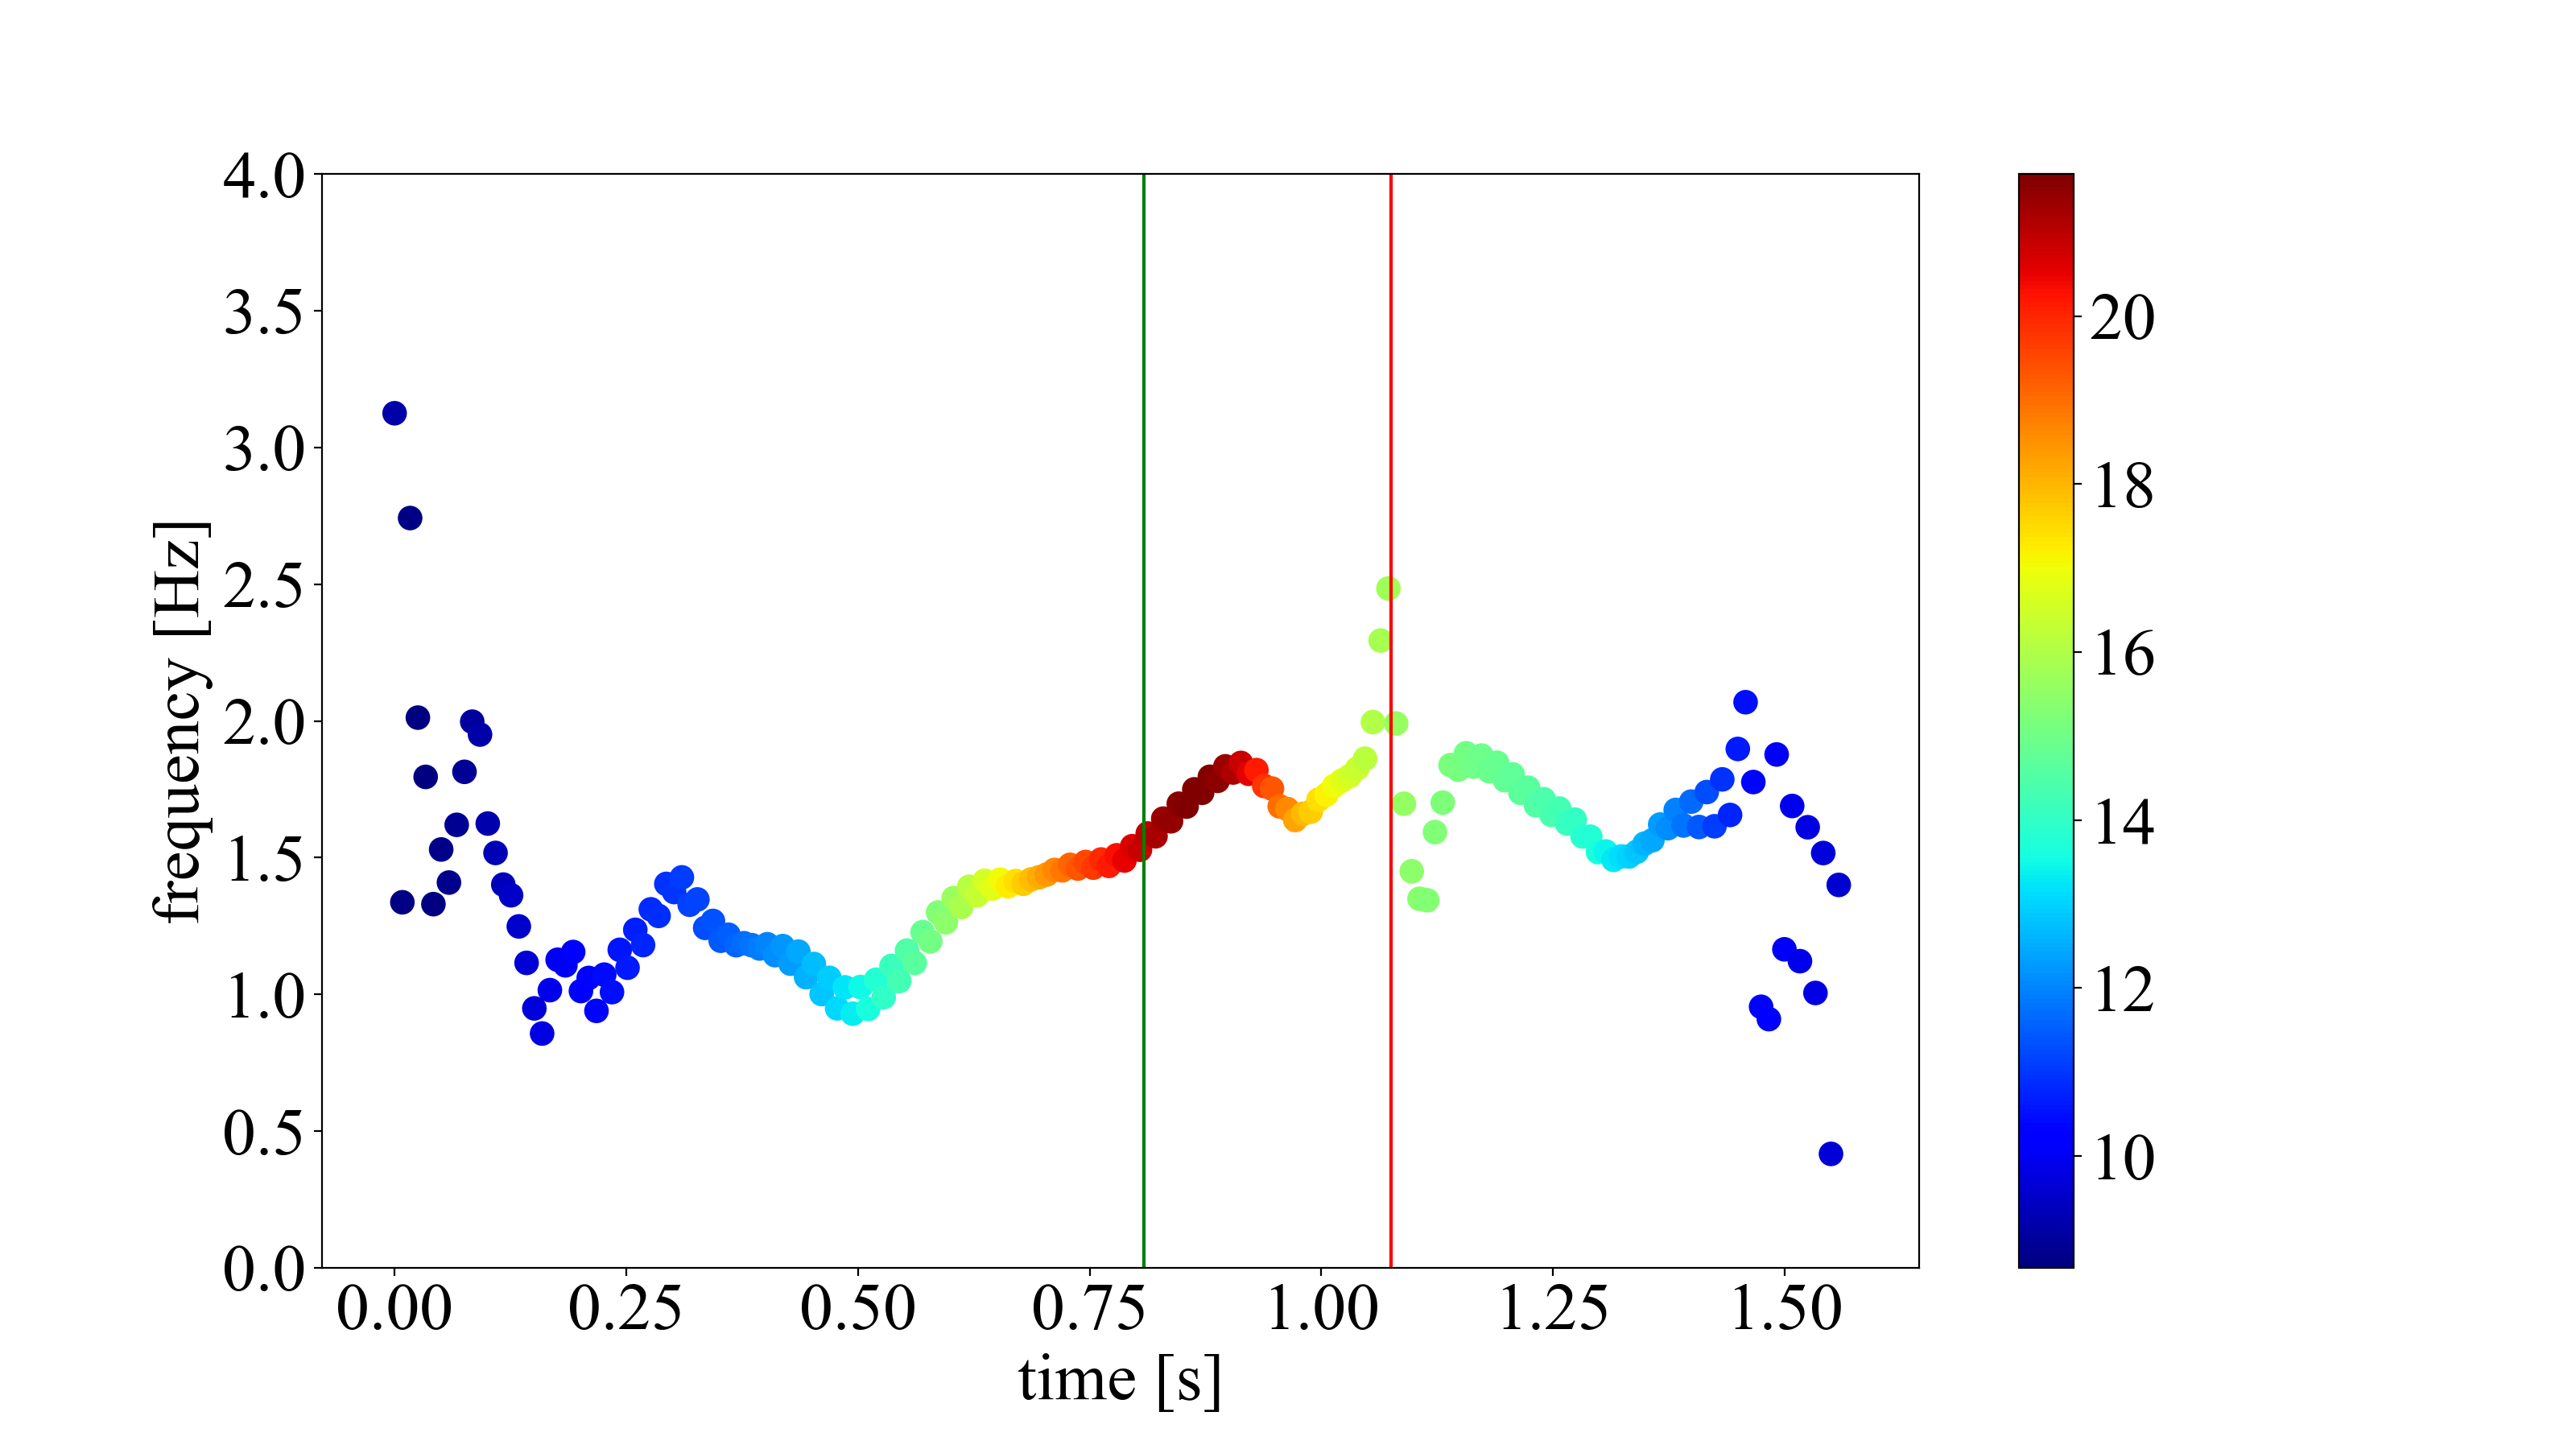
\includegraphics[width=8cm]{./images/opening_data/left_up_leg/IMF4.png}
                    (i)
                \end{center}
            \end{minipage}

            \begin{minipage}{0.5\hsize}
                \begin{center}
                    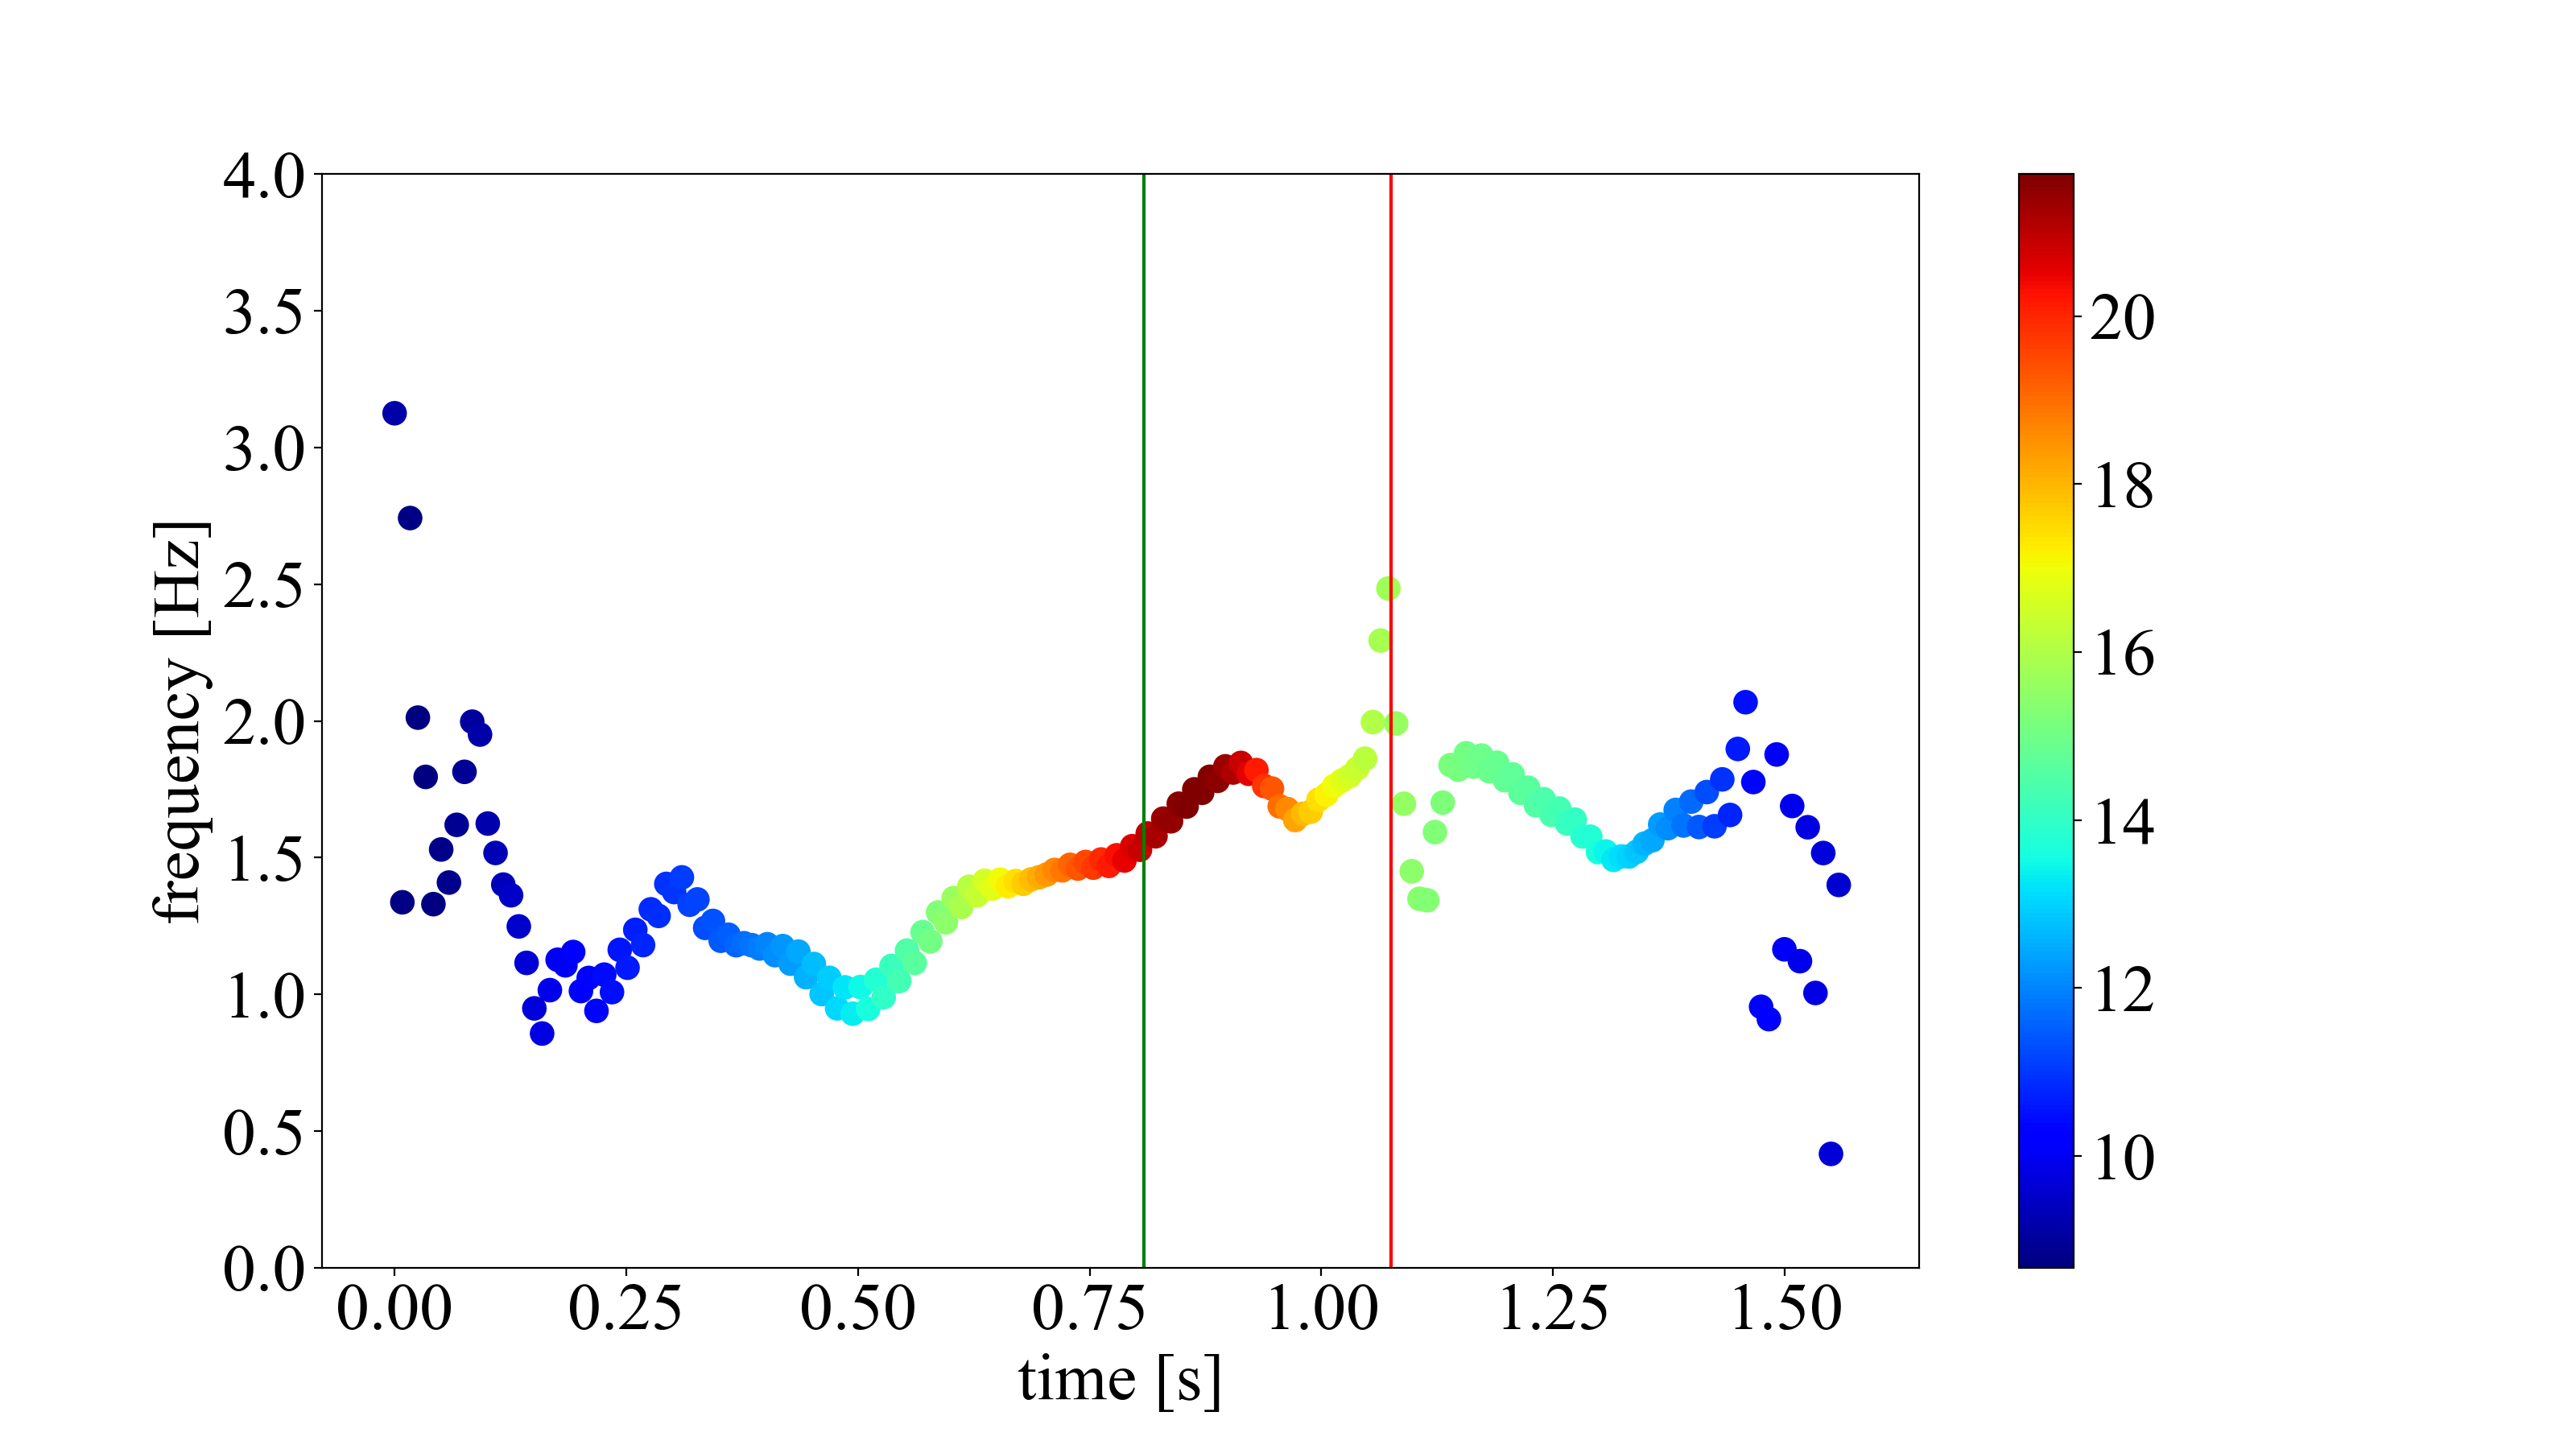
\includegraphics[width=8cm]{./images/opening_data/left_up_leg/IMF4.png}
                    (j)
                \end{center}
            \end{minipage}
        \end{tabular}
    \end{center}
    \caption{ストレート弾道,スライス弾道に飛球した左腿,左膝モーションIMF4のスペクトログラム.(g)はストレート弾道の左腿モーションIMF4.(h)はストレート弾道の左膝モーションIMF4.(i)はスライス弾道の左腿モーションIMF4.(h)はスライス弾道の左膝モーションIMF4.}
\end{figure}
